% Options for packages loaded elsewhere
\PassOptionsToPackage{unicode}{hyperref}
\PassOptionsToPackage{hyphens}{url}
\PassOptionsToPackage{dvipsnames,svgnames,x11names}{xcolor}
%
\documentclass[
  11pt,
  article]{jss}

\usepackage{amsmath,amssymb}
\usepackage{lmodern}
\usepackage{iftex}
\ifPDFTeX
  \usepackage[T1]{fontenc}
  \usepackage[utf8]{inputenc}
  \usepackage{textcomp} % provide euro and other symbols
\else % if luatex or xetex
  \usepackage{unicode-math}
  \defaultfontfeatures{Scale=MatchLowercase}
  \defaultfontfeatures[\rmfamily]{Ligatures=TeX,Scale=1}
\fi
% Use upquote if available, for straight quotes in verbatim environments
\IfFileExists{upquote.sty}{\usepackage{upquote}}{}
\IfFileExists{microtype.sty}{% use microtype if available
  \usepackage[]{microtype}
  \UseMicrotypeSet[protrusion]{basicmath} % disable protrusion for tt fonts
}{}
\makeatletter
\@ifundefined{KOMAClassName}{% if non-KOMA class
  \IfFileExists{parskip.sty}{%
    \usepackage{parskip}
  }{% else
    \setlength{\parindent}{0pt}
    \setlength{\parskip}{6pt plus 2pt minus 1pt}}
}{% if KOMA class
  \KOMAoptions{parskip=half}}
\makeatother
\usepackage{xcolor}
\setlength{\emergencystretch}{3em} % prevent overfull lines
\setcounter{secnumdepth}{-\maxdimen} % remove section numbering
% Make \paragraph and \subparagraph free-standing
\ifx\paragraph\undefined\else
  \let\oldparagraph\paragraph
  \renewcommand{\paragraph}[1]{\oldparagraph{#1}\mbox{}}
\fi
\ifx\subparagraph\undefined\else
  \let\oldsubparagraph\subparagraph
  \renewcommand{\subparagraph}[1]{\oldsubparagraph{#1}\mbox{}}
\fi


\providecommand{\tightlist}{%
  \setlength{\itemsep}{0pt}\setlength{\parskip}{0pt}}\usepackage{longtable,booktabs,array}
\usepackage{calc} % for calculating minipage widths
% Correct order of tables after \paragraph or \subparagraph
\usepackage{etoolbox}
\makeatletter
\patchcmd\longtable{\par}{\if@noskipsec\mbox{}\fi\par}{}{}
\makeatother
% Allow footnotes in longtable head/foot
\IfFileExists{footnotehyper.sty}{\usepackage{footnotehyper}}{\usepackage{footnote}}
\makesavenoteenv{longtable}
\usepackage{graphicx}
\makeatletter
\def\maxwidth{\ifdim\Gin@nat@width>\linewidth\linewidth\else\Gin@nat@width\fi}
\def\maxheight{\ifdim\Gin@nat@height>\textheight\textheight\else\Gin@nat@height\fi}
\makeatother
% Scale images if necessary, so that they will not overflow the page
% margins by default, and it is still possible to overwrite the defaults
% using explicit options in \includegraphics[width, height, ...]{}
\setkeys{Gin}{width=\maxwidth,height=\maxheight,keepaspectratio}
% Set default figure placement to htbp
\makeatletter
\def\fps@figure{htbp}
\makeatother
\newlength{\cslhangindent}
\setlength{\cslhangindent}{1.5em}
\newlength{\csllabelwidth}
\setlength{\csllabelwidth}{3em}
\newlength{\cslentryspacingunit} % times entry-spacing
\setlength{\cslentryspacingunit}{\parskip}
\newenvironment{CSLReferences}[2] % #1 hanging-ident, #2 entry spacing
 {% don't indent paragraphs
  \setlength{\parindent}{0pt}
  % turn on hanging indent if param 1 is 1
  \ifodd #1
  \let\oldpar\par
  \def\par{\hangindent=\cslhangindent\oldpar}
  \fi
  % set entry spacing
  \setlength{\parskip}{#2\cslentryspacingunit}
 }%
 {}
\usepackage{calc}
\newcommand{\CSLBlock}[1]{#1\hfill\break}
\newcommand{\CSLLeftMargin}[1]{\parbox[t]{\csllabelwidth}{#1}}
\newcommand{\CSLRightInline}[1]{\parbox[t]{\linewidth - \csllabelwidth}{#1}\break}
\newcommand{\CSLIndent}[1]{\hspace{\cslhangindent}#1}

\usepackage{booktabs}
\usepackage{longtable}
\usepackage{array}
\usepackage{multirow}
\usepackage{wrapfig}
\usepackage{float}
\usepackage{pdflscape}
\usepackage{tabu}
\usepackage{threeparttable}
\usepackage{threeparttablex}
\usepackage[normalem]{ulem}
\usepackage[utf8]{inputenc}
\usepackage{makecell}
\usepackage{xcolor}
\usepackage{placeins}


\newtheorem{definition}{Definition}
\usepackage{orcidlink,thumbpdf,lmodern}

\newcommand{\class}[1]{`\code{#1}'}
\newcommand{\fct}[1]{\code{#1()}}
\makeatletter
\@ifpackageloaded{tcolorbox}{}{\usepackage[many]{tcolorbox}}
\@ifpackageloaded{fontawesome5}{}{\usepackage{fontawesome5}}
\definecolor{quarto-callout-color}{HTML}{909090}
\definecolor{quarto-callout-note-color}{HTML}{0758E5}
\definecolor{quarto-callout-important-color}{HTML}{CC1914}
\definecolor{quarto-callout-warning-color}{HTML}{EB9113}
\definecolor{quarto-callout-tip-color}{HTML}{00A047}
\definecolor{quarto-callout-caution-color}{HTML}{FC5300}
\definecolor{quarto-callout-color-frame}{HTML}{acacac}
\definecolor{quarto-callout-note-color-frame}{HTML}{4582ec}
\definecolor{quarto-callout-important-color-frame}{HTML}{d9534f}
\definecolor{quarto-callout-warning-color-frame}{HTML}{f0ad4e}
\definecolor{quarto-callout-tip-color-frame}{HTML}{02b875}
\definecolor{quarto-callout-caution-color-frame}{HTML}{fd7e14}
\makeatother
\makeatletter
\makeatother
\makeatletter
\makeatother
\makeatletter
\@ifpackageloaded{caption}{}{\usepackage{caption}}
\AtBeginDocument{%
\ifdefined\contentsname
  \renewcommand*\contentsname{Table of contents}
\else
  \newcommand\contentsname{Table of contents}
\fi
\ifdefined\listfigurename
  \renewcommand*\listfigurename{List of Figures}
\else
  \newcommand\listfigurename{List of Figures}
\fi
\ifdefined\listtablename
  \renewcommand*\listtablename{List of Tables}
\else
  \newcommand\listtablename{List of Tables}
\fi
\ifdefined\figurename
  \renewcommand*\figurename{Figure}
\else
  \newcommand\figurename{Figure}
\fi
\ifdefined\tablename
  \renewcommand*\tablename{Table}
\else
  \newcommand\tablename{Table}
\fi
}
\@ifpackageloaded{float}{}{\usepackage{float}}
\floatstyle{ruled}
\@ifundefined{c@chapter}{\newfloat{codelisting}{h}{lop}}{\newfloat{codelisting}{h}{lop}[chapter]}
\floatname{codelisting}{Listing}
\newcommand*\listoflistings{\listof{codelisting}{List of Listings}}
\makeatother
\makeatletter
\@ifpackageloaded{caption}{}{\usepackage{caption}}
\@ifpackageloaded{subcaption}{}{\usepackage{subcaption}}
\makeatother
\makeatletter
\@ifpackageloaded{tcolorbox}{}{\usepackage[many]{tcolorbox}}
\makeatother
\makeatletter
\@ifundefined{shadecolor}{\definecolor{shadecolor}{rgb}{.97, .97, .97}}
\makeatother
\makeatletter
\makeatother
\ifLuaTeX
  \usepackage{selnolig}  % disable illegal ligatures
\fi
\IfFileExists{bookmark.sty}{\usepackage{bookmark}}{\usepackage{hyperref}}
\IfFileExists{xurl.sty}{\usepackage{xurl}}{} % add URL line breaks if available
\urlstyle{same} % disable monospaced font for URLs
\hypersetup{
  pdftitle={Making, Updating, and Querying Causal Models using CausalQueries},
  pdfauthor={Till Tietz; Lily Medina; Georgiy Syunyaev; Macartan Humphreys},
  colorlinks=true,
  linkcolor={blue},
  filecolor={Maroon},
  citecolor={Blue},
  urlcolor={Blue},
  pdfcreator={LaTeX via pandoc}}

%% -- Article metainformation (author, title, ...) -----------------------------

%% Author information
\author{Till Tietz~\orcidlink{0000-0002-2916-9059}\\WZB \And Lily
Medina\\UC Berkeley \AND Georgiy
Syunyaev~\orcidlink{0000-0002-4391-6313}\\Vanderbilt
University \And Macartan Humphreys~\orcidlink{0000-0001-7029-2326}\\WZB}
\Plainauthor{Till Tietz, Lily Medina, Georgiy Syunyaev, Macartan
Humphreys} %% comma-separated

\title{Making, Updating, and Querying Causal Models using
\texttt{CausalQueries}}
\Plaintitle{Making, Updating, and Querying Causal Models using
CausalQueries} %% without formatting

%% an abstract and keywords
\Abstract{A guide to the \proglang{R} package \texttt{CausalQueries} for
making, updating, and querying causal models}

%% at least one keyword must be supplied
\Keywords{causal models, stan, bayes}

%% publication information
%% NOTE: Typically, this can be left commented and will be filled out by the technical editor
%% \Volume{50}
%% \Issue{9}
%% \Month{June}
%% \Year{2012}
%% \Submitdate{2012-06-04}
%% \Acceptdate{2012-06-04}
%% \setcounter{page}{1}
%% \Pages{1--xx}

%% The address of (at least) one author should be given
%% in the following format:
\Address{
Till Tietz\\
IPI\\
Reichpietschufer 50\\
Berlin Germany\\
E-mail: \email{ttietz2014@gmail.com}\\
URL: \url{https://github.com/till-tietz}\\
\\~
Lily Medina\\
E-mail: \email{lily.medina@berkeley.edu}\\
URL: \url{https:/lilymedina.github.io/}\\
\\~
Georgiy Syunyaev\\
E-mail: \email{g.syunyaev@vanderbilt.edu}\\
URL: \url{https://gsyunyaev.com/}\\
\\~
Macartan Humphreys\\
E-mail: \email{macartan.humphreys@wzb.eu}\\
URL: \url{https://macartan.github.io/}\\
\\~

}

\begin{document}
\maketitle
\ifdefined\Shaded\renewenvironment{Shaded}{\begin{tcolorbox}[breakable, frame hidden, borderline west={3pt}{0pt}{shadecolor}, enhanced, interior hidden, boxrule=0pt, sharp corners]}{\end{tcolorbox}}\fi

\hypertarget{sec-intro}{%
\section{Introduction: Causal models}\label{sec-intro}}

\texttt{CausalQueries} is an \proglang{R} package that lets users make,
update, and query causal models. Users provide a statement that reports
a set of binary variables and the relations of causal ancestry between
them: which variables are direct causes of other variables, given the
other variables in the model. Once provided to \texttt{make\_model()},
\texttt{CausalQueries} generates a parameter vector that fully describes
a probability distribution over all possible types of causal relations
between variables (``causal types''), given the causal structure. Given
a prior over parameters and data over some or all nodes,
\texttt{update\_model()} deploys a \texttt{stan} model in order to
generate a posterior distribution over causal models. The function
\texttt{query\_model()} can then be used to ask any causal query of the
model, using either the prior distribution, the posterior distribution,
or a user-specified candidate vector of parameters.

In the next section we provide a short motivating example. We then
describe how the package relates to existing available software. Section
Section~\ref{sec-theory} gives an overview of the statistical model
behind the package. Sections Section~\ref{sec-make},
Section~\ref{sec-update}, and Section~\ref{sec-query} then describe the
main functionality for the major operations using the package. We
provide further computation details in the final section.

\hypertarget{motivating-example}{%
\section{Motivating example}\label{motivating-example}}

Before providing details on package functionality we illustrate these
three core functions by showing how to use \texttt{CuasalQueries} to
replicate the analysis in \citet{chickering1996clinician} (see also
\citet{ii2023}). \citet{chickering1996clinician} seek to draw inference
on causal effects in the presence of imperfect compliance. We have
access to an instrument \(Z\) (a randomly assigned prescription for
cholesterol medication), which is a cause of \(X\) (treatment uptake)
but otherwise unrelated to \(Y\) (cholesterol). We imagine we are
interested in three specific queries. The first is the average causal
effect of \(X\) on \(Y\). The second is the average effect for units for
which \(X=0\) and \(Y=0\). The last is the average treatment effect
\emph{for} ``compliers'': units for which \(X\) responds positively to
\(Z\). Thus two of these queries are conditional queries, with one
conditional on a counterfactual quantity.

Our data on \(Z\), \(X\), and \(Y\) is complete for all units and looks,
in compact form, as follows:

\begin{verbatim}
R> data("lipids_data")
R> 
R> lipids_data
\end{verbatim}

\begin{verbatim}
#>    event strategy count
#> 1 Z0X0Y0      ZXY   158
#> 2 Z1X0Y0      ZXY    52
#> 3 Z0X1Y0      ZXY     0
#> 4 Z1X1Y0      ZXY    23
#> 5 Z0X0Y1      ZXY    14
#> 6 Z1X0Y1      ZXY    12
#> 7 Z0X1Y1      ZXY     0
#> 8 Z1X1Y1      ZXY    78
\end{verbatim}

With \texttt{CausalQueries}, you can create the model, input data to
update it, and then query the model for results.

\begin{verbatim}
R> make_model("Z -> X -> Y; X <-> Y") |>
+  update_model(lipids_data, refresh = 0) |>
+  query_model(query = "Y[X=1] - Y[X=0]",
+              given = c("All",  "X==0 & Y==0", "X[Z=1] > X[Z=0]"),
+              using = "posteriors") 
\end{verbatim}

\hypertarget{tbl-lipids}{}
\begin{table}
\caption{\label{tbl-lipids}Replication of . }\tabularnewline

\centering
\resizebox{\linewidth}{!}{
\begin{threeparttable}
\begin{tabular}{cccccc}
\toprule
query & given & mean & sd & cred.low.2.5\% & cred.high.97.5\%\\
\midrule
Y[X=1] - Y[X=0] & - & 0.56 & 0.10 & 0.38 & 0.73\\
Y[X=1] - Y[X=0] & X==0 \& Y==0 & 0.64 & 0.15 & 0.38 & 0.89\\
Y[X=1] - Y[X=0] & X[Z=1] > X[Z=0] & 0.70 & 0.05 & 0.60 & 0.80\\
\bottomrule
\end{tabular}
\begin{tablenotes}
\small
\item Rows 1 and 2 replicate results in \citet{chickering1996clinician}; row 3 returns inferences for complier average effects.
\end{tablenotes}
\end{threeparttable}}
\end{table}

The output is a data frame with estimates, posterior standard
deviations, and credibility intervals. For example the data frame
produced by the code above is shown in Table~\ref{tbl-lipids}.

As we describe below the same basic procedure of making, updating, and
querying models, can be used (up to computational constraints) for
arbitrary causal models, for different types of data structures, and for
all causal queries that can be posed of the causal model.

\hypertarget{connections-to-existing-packages}{%
\section{Connections to existing
packages}\label{connections-to-existing-packages}}

The literature on causal inference and its software ecosystem are rich
and expansive; spanning the social and natural sciences as well as
computer science and applied mathematics. In the interest of clarity we
thus briefly contextualize \texttt{CausalQueries\textquotesingle{}}
scope and functionality within the subset of the causal inference domain
addressing the evaluation of causal queries on causal models encoded as
directed acyclic graphs (DAGs) or structural equation models (SEMs). We
provide a brief tabular overview of relevant software and discuss key
connections, advantages and disadvantages with respect to
\texttt{CausalQueries} in turn.

\begin{longtable}[]{@{}
  >{\raggedright\arraybackslash}p{(\columnwidth - 8\tabcolsep) * \real{0.1574}}
  >{\raggedright\arraybackslash}p{(\columnwidth - 8\tabcolsep) * \real{0.1777}}
  >{\raggedright\arraybackslash}p{(\columnwidth - 8\tabcolsep) * \real{0.1168}}
  >{\raggedright\arraybackslash}p{(\columnwidth - 8\tabcolsep) * \real{0.1320}}
  >{\centering\arraybackslash}p{(\columnwidth - 8\tabcolsep) * \real{0.4010}}@{}}
\toprule()
\begin{minipage}[b]{\linewidth}\raggedright
Software
\end{minipage} & \begin{minipage}[b]{\linewidth}\raggedright
Source
\end{minipage} & \begin{minipage}[b]{\linewidth}\raggedright
Language
\end{minipage} & \begin{minipage}[b]{\linewidth}\raggedright
Availability
\end{minipage} & \begin{minipage}[b]{\linewidth}\centering
Scope
\end{minipage} \\
\midrule()
\endhead
\textbf{autobounds} & \citet{Duarte2023autobounds} & \textbf{Python} &
not readily installable & \begin{minipage}[t]{\linewidth}\centering
\begin{itemize}
\tightlist
\item
  bounding causal effects
\item
  partial identification
\item
  DAG canonicalization
\item
  binary data
\end{itemize}
\end{minipage} \\
\textbf{causalnex} & \citet{Beaumont2021causalnex} & \textbf{Python} &
pip installable & \begin{minipage}[t]{\linewidth}\centering
\begin{itemize}
\tightlist
\item
  causal structure learning
\item
  querying marginal distributions
\item
  discrete data
\end{itemize}
\end{minipage} \\
\textbf{causaloptim} & \citet{sachs2023causaloptim} & \textbf{R} & CRAN
& \begin{minipage}[t]{\linewidth}\centering
\begin{itemize}
\tightlist
\item
  bounding causal effects
\item
  non-identified queries
\item
  binary data
\end{itemize}
\end{minipage} \\
\textbf{pclag} & \citet{kalisch2012pclag} & \textbf{R} & CRAN &
\begin{minipage}[t]{\linewidth}\centering
\begin{itemize}
\tightlist
\item
  causal structure learning
\item
  ATEs under linear conditional expectations and no hidden selection
\end{itemize}
\end{minipage} \\
\bottomrule()
\end{longtable}

One of the most comprehensive pieces of software in the causal modeling
domain is \texttt{causalnex}. It provides a feature rich and highly
optimized set of tools to learn, update and query causal models using
discrete data. While avoiding the rich model parameterization via
principal strata (nodal types) employed by \texttt{CausalQueries},
allows \texttt{causalnex} to easily handle non-binary data and scale to
large causal models; it substantially restricts the set of possible
queries that can be evaluated and prior knowledge that can be specified
on models. \texttt{causalnex} is in this sense akin to machine learning
approaches to causal inference, focusing on causal structure learning in
variable rich but potentially domain knowledge poor settings and the
evaluation of simple queries over marginal distributions on learned
DAGs. The rich model structure employed by \texttt{CausalQueries} by
contrast makes it highly suited to problems where answers to complex
causal queries are sought in relatively more domain knowledge abundant
settings. Like \texttt{causalnex} \texttt{pclag} places particular
emphasis on causal structure learning, utilizing the resultant DAGs to
recover ATEs across all learned markov-equivalent classes implied by
observed data that satisfy linearity of conditional expectations. This
approach again is far more restrictive than \texttt{CausalQueries} in
the the DAGs and queries it allows. The methods bearing the highest
resemblance to \texttt{CausalQueries} with respect to model definition
are \texttt{autobounds} and \texttt{causaloptim}. Dealing with binary
causal models, their definitions of principal strata (nodal types) and
the resultant set of causal relations on the DAG (causal types) are
identical to those of \texttt{CausalQueries}. Differences in model
definition arise only with respect to disturbance terms and confounding
being defined implicitly via main nodes and edges in
\texttt{CausalQueries} vs explicitly via separate disturbance nodes in
\texttt{autobounds} and \texttt{causaloptim}. A key consequence of this
is that while \texttt{CausalQueries} assumes canonical form for input
DAGs, \texttt{autobounds} and \texttt{causaloptim} facilitate
cannonicalization. The essential difference between the methods;
however, lies in their approach to evaluating queries. While
\texttt{autobounds} and \texttt{causaloptim} conceptualize query
evaluation as constrained polynomial and linear optimization problems
respectively, \texttt{CausalQueries} utilizes Bayesian inference to
generate a posterior over the causal model (\citet{zhang2022pci} propose
a Bayesian model similar to \texttt{CausalQueries} but provide no
software implementation). The polynomial and linear programming approach
to querying is in principle suited to handling somewhat larger causal
models, though given their similarity in model parameterization
\texttt{autobounds}, \texttt{causaloptim} and \texttt{CausalQueries}
face similar constraints induced by parameter spaces expanding rapidly
with model size. The Bayesian approach to model updating and querying
holds the major efficiency advantage that a model can be updated once
and queried infinitely, while expensive optimization runs are required
for each separate query in \texttt{autobounds} and \texttt{causaloptim}.
This in addition to allowing for full Bayesian inference and the ablity
to generate complete posteriors over causal queries instead of bounds is
a major advantage of \texttt{CausalQueries}. It is further unclear
whether polynomial and linear optimization can effectively handle
complex causal queries with nested do operations. \texttt{CausalQueries}
fundamentally combines the feature richness of more general causal
inference software with the modeling and querying flexibility afforded
by rich model parameterizations and fully Bayesian inference.

The particular strength of \texttt{CausalQueries} is to allow users to
specify arbitrary DAGs, arbitrary queries over nodes in those DAGs, and
use the same canonical procedure to learn about those queries whether or
not the queries are identified. Thus in principle if researchers are
interest in learning about a quantity like the local average treatment
effect and their model in fact satisfies the conditions in
\citet{angrist1996identification}, then updating will recover valid
estimates even if researchers are unaware that the local average
treatment effect is identified and are ignorant of the estimation
procedure proposed by \citet{angrist1996identification}.

There are two broad limitation on the sets of models handled natively by
\texttt{CausalQueries}. First \texttt{CausalQueries} is designed for
models with a relatively small number over binary nodes. Because there
is no compromise made on the space of possible causal relations implied
by a given model, the parameter space grows very rapidly with the
complexity of the causal model. The complexity also depends on the
causal structure and grows rapidly with the number of parents affecting
a given child. A chain model of the form
\(A \rightarrow B \rightarrow C \rightarrow D \rightarrow E\) has just
40 parameters. A model in which \(A, B, C, D\) are all direct of \(E\)
has 65544 parameters. Moving from binary to non binary nodes has similar
effects. The restriction to binary nodes is for computational and not
conceptual reasons. In fact it is possible to employ
\texttt{CausalQueries} to answer queries from models with nonbinary
nodes but in general the computational costs make analysis of these
model prohibitive.\footnote{For more on computation constraints and
  strategies to update and query large models see the associated package
  \texttt{CausalQueriesTools}. The core approach used here is to divde
  large causal models into modules, update on modules and reassemble to
  pose queries.}

Second, the package is geared for learning about populations from
samples of units that are independent of each other and are
independently randomly sampled from populations. Thus the basic set up
does not address problems of sampling, clustering, hierarchical
structures, or purposive sampling, for example. The broader framework
can however be used for these purposes (see section 9.4 of
\citet{ii2023}). The target of inference is usually case level
quantities or population quantities and not sample quantities.

\hypertarget{sec-theory}{%
\section{Statistical model}\label{sec-theory}}

The core conceptual framework is described in Pearl's \emph{Causality}
\citep{pearl2009causality} but can be summarized as follows (using the
notation used in \citet{ii2023}):

\begin{definition}
  
  A ``\textbf{causal model}'' is:
  \begin{enumerate}
    \item an ordered collection of "endogenous nodes" $Y = \{Y_1, Y_2, \dots, Y_n\}$
    \item an ordered collection of "exogenous nodes" $\Theta = \{\theta^{Y_1}, \theta^{Y_1}, \dots, \theta^{Y_n}\}$
    \item a collection of functions $F = \{f_{Y_1}, f_{Y_2}, \dots, f_{Y_n}\}$ specifying, for each node $j$, how outcome $y_j$ depends on $\theta_j$ and realizations of endogenous nodes prior to $j$.
    \item a probability distribution over $\Theta$, $\lambda$
  \end{enumerate}
  
\end{definition}

In the usual case we take the endogenous nodes to be binary.\footnote{\texttt{CausalQueries}
  can be used also to analyse non binary data though with a cost of
  greatly increased complexity. See section 9.4.1 of \citet{ii2023} for
  an approach that codes non binary data as a profile of outcomes on
  multiple binary nodes.} When we specify a causal structure we specify
which endogenous nodes are (possibly) direct causes of a node, \(Y_j\),
given other nodes in the model. These nodes are called the parents of
\(Y_j\), \(PA_j\) (we use upper case \(PA_j\) to indicate the collection
of nodes and lower case \(pa_j\) to indicate a particular set of values
that these nodes might take on). With discrete valued nodes, it is
possible to identify all possible ways that a node might respond to its
parents. We refer to the ways that a node responds and the nodes ``nodal
type.'' The set of nodal types corresponds to principal strata familiar,
for instance, in the study of instrumental variables
\citep{frangakis2002principal}.

If node \(Y_i\) can take on \(k_i\) possible values then the set of
possible values that can be taken on by parents of \(j\) is
\(m :=\prod_{i\in PA_j}k_i\). Then there are \(k_j^{m}\) different ways
that a node might respond to its parents. In the case of binary nodes
this becomes \(2^{\left(2^{|PA_j|}\right)}\). Thus for an endogenous
node with no parents there are 2 nodal types, for a binary node with one
binary parent there are four types, for a binary node with 2 parents
there are 16, and so on.

The set of all possible causal reactions of a given unit to all possible
values of parents is then given by its collection of nodal types at each
node. We call this collection a unit's ``causal type'', \(\theta\).

The approach used by \texttt{CausalQueries} is to let the domain of
\(\theta^{Y_j}\) be coextensive with the number of nodal types for
\(Y_j\). Function \(f^j\) then determines the value of \(y\) by simply
reporting the value of \(Y_j\) implied by the nodal type and the values
of the parents of \(Y_j\). Thus if \(\theta^j_{pa_j}\) is the value for
\(j\) when parents have values \(pa_j\), then we have simply that
\(f_{y_j}(\theta^{j}, pa_j) = \theta^j_{pa_j}\). The practical
implication is that, given the causal structure, learning about the
model reduces to learning about the distribution, \(\lambda\), over the
nodal types.

In cases in which there is no unobserved confounding, we take the
probability distributions over the nodal types for different nodes to be
independent: \(\theta^i \perp\!\!\! \perp \theta^j, i\neq j\). In this
case we use a categorical distribution to specify the
\({\lambda^j}' := \Pr(\theta^j = {\theta^j}')\). From independence then
we have that the probability of a given causal type \(\theta'\) is
simply \(\prod_{i=1}^n {\lambda^i}'\).

In cases in which there is confounding, the logic is essentially the
same except that we need to specify enough parameters to capture the
joint distribution over nodal types for different nodes.

We make use of the causal structure to simplify. As an example, for the
lipids model, the full joint distribution of nodal types can be
simplified as in Equation~\ref{eq-join}.

\begin{equation}\protect\hypertarget{eq-join}{}{
\Pr(\theta^Z = \theta^Z_1, \theta^X = \theta^X_{10}, \theta^Y = \theta^Y_{11}) = 
\Pr(\theta^Z = \theta^Z_1)\Pr(\theta^X = \theta^X_{10})\Pr(\theta^Y = \theta^Y_{11}|\theta^X = \theta^X_{10})
}\label{eq-join}\end{equation}

And so for this model \(\lambda\) would include parameters that
represent \(\Pr(\theta^Z)\) and \(\Pr(\theta^X)\) but also the
conditional probability \(\Pr(\theta^Y|\theta^X)\):

\begin{equation}\protect\hypertarget{eq-join2}{}{
\Pr(\theta^Z = \theta^Z_1, \theta^X = \theta^X_{10}, \theta^Y = \theta^Y_{11}) = 
\lambda^Z_1\lambda^X_{10}\lambda^{Y|\theta^X_{10}}_{11}
}\label{eq-join2}\end{equation}

Representing beliefs \emph{over causal models} thus requires specifying
a probability distribution over \(\lambda\). This might be a degenerate
distribution if users want to specify a particular model.
\texttt{CausalQueries} allows users to specify parameters, \(\alpha\) of
a Dirichlet distribution over \(\lambda\). If all entries of \(\alpha\)
are 0.5 this corresponds to Jeffrey's priors. The default behavior is
for \texttt{CausalQueries} to assume a uniform distribution -- that is,
that all nodal types are equally likely -- which corresponds to
\(\alpha\) being a vector of 1s.

Updating is then done with respect to beliefs over \(\lambda\). In the
Bayesian approach we have simply:

\[p(\lambda'|D) = \frac{p(D|\lambda')p(\lambda')}{\int_{\lambda^{''}} p(D|\lambda'')p(\lambda'')}\]

\(p(D|\lambda')\) is calculated under the assumption that units are
exchangeable and independently drawn, and of course. In practice this
means that the probability that two units have causal types \(\theta_i\)
and \(\theta_j\) is simply \(\lambda'_i\lambda'_j\). Since a causal type
fully determines an outcome vector \(d = \{y_1, y_2,\dots,y_n\}\), the
probability of a given outcome (``event''), \(w_d\), is given simply by
the probability that the causal type is among those that yield outcome
\(d\). Thus from \(\lambda'\) we can calculate a vector of event
probabilities, \(w(\lambda)\), for each vector of outcomes, and under
independence we have:

\[D \sim \text{Mulitinomial}(w(\lambda), N)\]

Thus for instance in the case of a \(X \rightarrow Y\) model, and
letting \(w_{xy}\) denote the probability of a data type \(X=x, Y=y\),
the event probabilities are:

\[w(\lambda) = \left\{\begin{array}{ccc} w_{00} & = & \lambda^X_0(\lambda^Y_{00} + \lambda^Y_{01})\\ 
w_{01} & = & \lambda^X_0(\lambda^Y_{11} + \lambda^Y_{10})\\
w_{10} & = & \lambda^X_1(\lambda^Y_{00} + \lambda^Y_{10})\\
w_{11} & = & \lambda^X_1(\lambda^Y_{11} + \lambda^Y_{01})\end{array} \right.\]

For concreteness: table \citet{lipidspar} illustrates key values for the
lipids model. We see here that we have two types for node \(Z\), four
for \(X\) (representing the strata familiar from instrumental variables
analysis: never takers, always takers, defiers, and compliers) and 4 for
\(Y\). For \(Z\) and \(X\) we have parameters corresponding to
probability of these nodal types. For instance \texttt{Z.0} is the
probability that \(Z=1\). \texttt{Z.1} is the complementary probability
that \(Z=1\). Things are little more complicated for distributions on
nodal types for \(Y\) however: because of confounding between \(X\) and
\(Y\) we have parameters that capture the conditional probability of the
nodal types for \(Y\) \emph{given} the nodal types for \(X\). We see
there are four sets of these parameters.

\begin{table}

\caption{Nodal types and parameters for Lipids model}
\centering
\begin{tabular}[t]{ccccc}
\toprule
node & nodal\_type & param\_set & param\_names & param\_value\\
\midrule
Z & 0 & Z & Z.0 & 0.71\\
Z & 1 & Z & Z.1 & 0.29\\
X & 00 & X & X.00 & 0.36\\
X & 10 & X & X.10 & 0.03\\
X & 01 & X & X.01 & 0.51\\
X & 11 & X & X.11 & 0.10\\
Y & 00 & Y.X.00 & Y.00\_X.00 & 0.43\\
Y & 10 & Y.X.00 & Y.10\_X.00 & 0.08\\
Y & 01 & Y.X.00 & Y.01\_X.00 & 0.34\\
Y & 11 & Y.X.00 & Y.11\_X.00 & 0.15\\
Y & 00 & Y.X.01 & Y.00\_X.01 & 0.43\\
Y & 10 & Y.X.01 & Y.10\_X.01 & 0.05\\
Y & 01 & Y.X.01 & Y.01\_X.01 & 0.39\\
Y & 11 & Y.X.01 & Y.11\_X.01 & 0.13\\
Y & 00 & Y.X.10 & Y.00\_X.10 & 0.24\\
Y & 10 & Y.X.10 & Y.10\_X.10 & 0.45\\
Y & 01 & Y.X.10 & Y.01\_X.10 & 0.12\\
Y & 11 & Y.X.10 & Y.11\_X.10 & 0.19\\
Y & 00 & Y.X.11 & Y.00\_X.11 & 0.61\\
Y & 10 & Y.X.11 & Y.10\_X.11 & 0.11\\
Y & 01 & Y.X.11 & Y.01\_X.11 & 0.03\\
Y & 11 & Y.X.11 & Y.11\_X.11 & 0.25\\
\bottomrule
\end{tabular}
\end{table}

The final column shows a sample set of parameter values. Together the
parameters describe a full joint probability distribution over types for
\(Z\), \(X\) and \(Y\) that is faithful to the graph.

From these we can calculate the probability of each data type. For
instance the probability of data type \(Z=0, X=0, Y=0\) is:

\[w_{000}=\Pr(Z=0, X=0, Y=0) = \lambda^Z_0\left(\lambda^X_{00}(\lambda^{Y|\lambda^X_{00}}_{00}+\lambda^{Y|\lambda^X_{00}}_{01}) + \lambda^X_{01}(\lambda^{Y|\lambda^X_{01}}_{00}+\lambda^{Y|\lambda^X_{01}}_{01})\right)\]
In practice \texttt{CausalQueries} uses a matrix \texttt{parmap} that
maps from parameters into data types.

The value of the \texttt{CausalQueries} package is to allow users to
specify \emph{arbitrary} models of this form, figure out all the implied
nodal types and causal types, and then update given priors and data by
calculating event probabilities implied by all possible parameter
vectors and in turn the likelihood of the data given the model. In
addition, the package allows for arbitrary querying of a model to assess
the values of estimands of interest that a re function of the values or
counterfactual values of nodes conditional on values or counterfactual
values of nodes.

In the next sections we review key functionality for making, updating
and querying causal models.

\hypertarget{sec-make}{%
\section{Making models}\label{sec-make}}

A model is defined in one step in \texttt{CausalQUeries} using a
\texttt{dagitty} syntax in which the structure of the model is provided
as a statement.

For instance:

\begin{verbatim}
R> model <- make_model("X -> M -> Y <- X")
\end{verbatim}

The statement in quotes,
\texttt{"X\ -\textgreater{}\ M\ -\textgreater{}\ Y\ \textless{}-\ X"},
provides the names of nodes. An arrow (``\texttt{-\textgreater{}}'' or
``\texttt{\textless{}-}'') connecting nodes indicates that one node is a
potential cause of another, i.e.~whether a given node is a ``parent'' or
``child'' of another.

Formally a statement like this is interpreted as:

\begin{enumerate}
\def\labelenumi{\arabic{enumi}.}
\item
  Functional equations:

  \begin{itemize}
  \tightlist
  \item
    \(Y = f(M, X, \theta^Y)\)
  \item
    \(M = f(X, \theta^M)\)
  \item
    \(X = \theta^X\)
  \end{itemize}
\item
  Distributions on \(\Theta\):

  \begin{itemize}
  \tightlist
  \item
    \(\Pr(\theta^i = \theta^i_k) = \lambda^i_k\)
  \end{itemize}
\item
  Independence assumptions:\\

  \begin{itemize}
  \tightlist
  \item
    \(\theta_i \perp\!\!\! \perp \theta_j, i\neq j\)
  \end{itemize}
\end{enumerate}

where function \(f\) maps from the set of possible values of the parents
of \(i\) to values of node \(i\) given \(\theta^i\) as described above.

In addition, as we did in the \citet{chickering1996clinician} example,
it is possible to use two headed arrows
(\texttt{\textless{}-\textgreater{}}) to indicate ``unobserved
confounding'', that is, the presence of an unobserved variable that
might influence observed variables. In this case condition 3 above is
relaxed and the exogeneous nodes associated with confounded variables
have a joint distribution. We describe how this is done in greater
detail in section \textbf{?@sec-confounding}.

\hypertarget{graphing}{%
\subsection{Graphing}\label{graphing}}

Plotting the model can be useful to check that you have defined the
structure of the model correctly. \texttt{CausalQueries} provides simple
graphing tools that draw on functionality from the \texttt{dagitty},
\texttt{ggplot2}, and \texttt{ggdag} packages.

Once defined, a model can be graphed by calling the \texttt{plot()}
method defined for the objects with class \texttt{causal\_model}
produced by \texttt{make\_model()} function.

\begin{verbatim}
R> make_model("X -> M -> Y <- X; Z -> Y") |>
+  plot()
\end{verbatim}

Alternatively you can provide a number of options to the \texttt{plot()}
call that will be passed to \texttt{CausalQueries:::plot\_dag} via the
method.

\begin{verbatim}
R> make_model("X -> M -> Y <- X; Z -> Y") |>
+  plot(x_coord = 1:4,
+       y_coord = c(1.5,2,1,2),
+       textcol = "white",
+       textsize = 3,
+       shape = 18,
+       nodecol = "grey",
+       nodesize = 12)
\end{verbatim}

The graphs produced by the two calls above are shown in
Figure~\ref{fig-plots}. In both cases the resulting plot will have class
\texttt{c("gg",\ "ggplot")} and so will accept any additional
modifications available via \texttt{ggplot2} package.

\begin{figure}

\begin{minipage}[t]{0.50\linewidth}

{\centering 

\raisebox{-\height}{

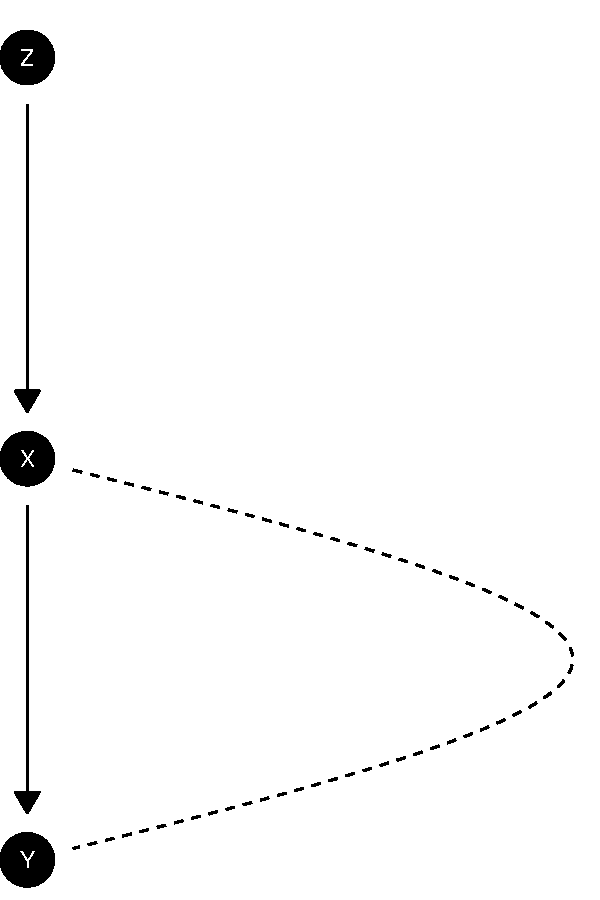
\includegraphics{paper_files/figure-pdf/fig-plots-1.pdf}

}

}

\subcaption{\label{fig-plots-1}Without options}
\end{minipage}%
%
\begin{minipage}[t]{0.50\linewidth}

{\centering 

\raisebox{-\height}{

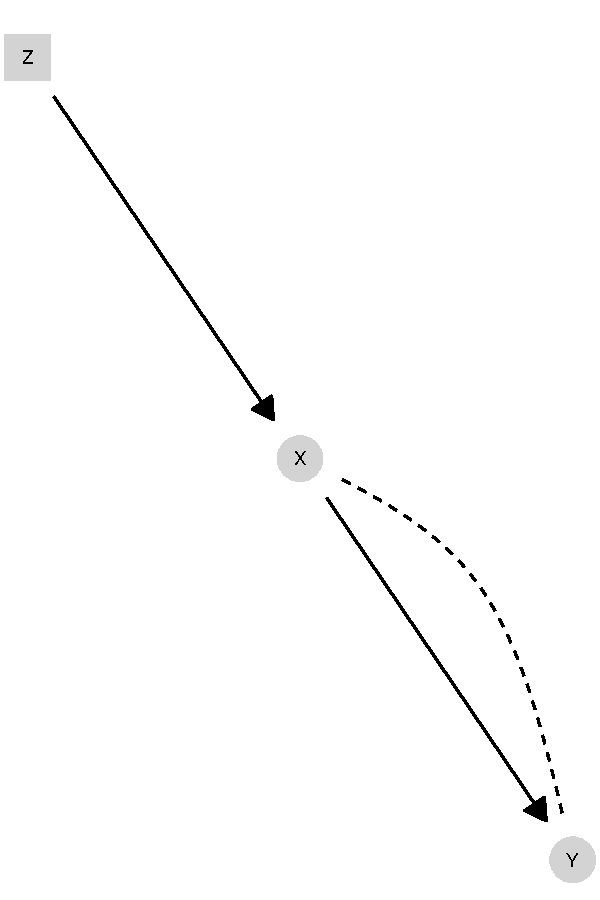
\includegraphics{paper_files/figure-pdf/fig-plots-2.pdf}

}

}

\subcaption{\label{fig-plots-2}With options}
\end{minipage}%

\caption{\label{fig-plots}Examples of model graphs.}

\end{figure}

\hypertarget{model-characterization}{%
\subsection{Model characterization}\label{model-characterization}}

When a model is defined, a set of objects is generated. These are the
key quantities that are used for all inference. The table below
summarizes the core components of a model, providing a brief explanation
for each one.

The first element is a \texttt{statement} which defines how the nodes in
the model are related, specified by the user using \texttt{dagitty}
syntax. The second element, \texttt{dag}, is a dataframe that outlines
the implied parent-child relationships within the model. \texttt{nodes}
is simply a list of the names of the implied nodes in the model. Lastly,
\texttt{parents\_df,} is a table listing the nodes, indicating if they
are ``root'' nodes (notes with no parents among the set of specified
nodes), and showing how many parents each node has.

The model includes additional elements, \texttt{nodal\_types,}
\texttt{parameters\_df,} and \texttt{causal\_types,} which we explain
later in detail.

\begin{longtable}[]{@{}
  >{\raggedright\arraybackslash}p{(\columnwidth - 2\tabcolsep) * \real{0.3000}}
  >{\raggedright\arraybackslash}p{(\columnwidth - 2\tabcolsep) * \real{0.7000}}@{}}
\caption{Core Elements of a Causal Model.}\tabularnewline
\toprule()
\begin{minipage}[b]{\linewidth}\raggedright
Element
\end{minipage} & \begin{minipage}[b]{\linewidth}\raggedright
Description
\end{minipage} \\
\midrule()
\endfirsthead
\toprule()
\begin{minipage}[b]{\linewidth}\raggedright
Element
\end{minipage} & \begin{minipage}[b]{\linewidth}\raggedright
Description
\end{minipage} \\
\midrule()
\endhead
\texttt{statement} & A character string that describes directed causal
relations between variables in a causal model, where arrows denote that
one node is a potential cause of another. \\
\texttt{dag} & A data frame with columns `parent' and `children'
indicating how nodes relate to each other. \\
\texttt{nodes} & A list containing the nodes in the model. \\
\texttt{parents\_df} & A table listing nodes, whether they are root
nodes or not, and the number of parents they have. \\
\texttt{nodal\_types} & A list with the nodal types in the model. See
Section~\ref{sec-nodal-types} for more details. \\
\texttt{parameters\_df} & A data frame linking the model's parameters
with the nodal types of the model, as well as the family to which they
belong. See Section~\ref{sec-param-df} for more details. \\
\texttt{causal\_types} & A data frame listing causal types and the nodal
types that produce them. (See Causal Types Section) \\
\bottomrule()
\end{longtable}

After updating a model, two additional components are attached to it:

\begin{itemize}
\item
  A posterior distribution of the parameters in the model, generated by
  stan. This distribution reflects the updated parameter values.
\item
  A list of objects, which we refer to as \texttt{stan\_objects}. The
  \texttt{stan\_objects} will, at a minimum, include the distribution of
  nodal types and the data used for updating the model
\end{itemize}

Optionally, users can choose whether to keep and append additional
elements to the \texttt{stan\_objects.} For instance, they can specify
whether to include \texttt{w}, which maps parameters to event
probabilities, as well as the \texttt{stanfit} object, the output
generated by stan

The table below summarizes the objects attached to the model after
updating.

\begin{longtable}[]{@{}
  >{\raggedright\arraybackslash}p{(\columnwidth - 2\tabcolsep) * \real{0.3000}}
  >{\raggedright\arraybackslash}p{(\columnwidth - 2\tabcolsep) * \real{0.7000}}@{}}
\caption{Additional Elements.}\tabularnewline
\toprule()
\begin{minipage}[b]{\linewidth}\raggedright
Element
\end{minipage} & \begin{minipage}[b]{\linewidth}\raggedright
Description
\end{minipage} \\
\midrule()
\endfirsthead
\toprule()
\begin{minipage}[b]{\linewidth}\raggedright
Element
\end{minipage} & \begin{minipage}[b]{\linewidth}\raggedright
Description
\end{minipage} \\
\midrule()
\endhead
\texttt{posterior\_distribution} & The posterir distribution of the
updated parameters generated by stan. \\
\texttt{stan\_objects} & A list of objects, including, at a minimum,
\texttt{type\_distribution} and \texttt{data}. \\
\texttt{data} & The data used for updating the model, appended to
\texttt{stan\_objects.} \\
\texttt{type\_distribution} & The updated distribution of the nodal
types, appended to \texttt{stan\_objects.} \\
\texttt{w} & A mapping from parameters to event probabilities,
optionally appended to \texttt{stan\_objects.} \\
\texttt{stan\_fit} & The \texttt{stanfit} object generated by stan. This
is optionally appended to \texttt{stan\_objects.} \\
\bottomrule()
\end{longtable}

\hypertarget{sec-param-df}{%
\subsubsection{Parameters data frame}\label{sec-param-df}}

When a model is created, \texttt{CausalQueries} attaches a ``parameters
data frame'' which keeps track of model parameters, which belong
together in a family, and how they relate to causal types. This becomes
especially important for more complex models with confounding that might
involve more complicated mappings between parameters and nodal types. In
the case with no confounding the nodal types \emph{are} the parameters;
in cases with confounding there are generally more parameters than nodal
types.

For instance:

\begin{verbatim}
R> make_model("X -> Y")$parameters_df
\end{verbatim}

\begin{verbatim}
#> # A tibble: 6 x 8
#>   param_names node    gen param_set nodal_type given param_value priors
#>   <chr>       <chr> <int> <chr>     <chr>      <chr>       <dbl>  <dbl>
#> 1 X.0         X         1 X         0          ""           0.5       1
#> 2 X.1         X         1 X         1          ""           0.5       1
#> 3 Y.00        Y         2 Y         00         ""           0.25      1
#> 4 Y.10        Y         2 Y         10         ""           0.25      1
#> 5 Y.01        Y         2 Y         01         ""           0.25      1
#> 6 Y.11        Y         2 Y         11         ""           0.25      1
\end{verbatim}

\hypertarget{tbl-params-df}{}
\begin{table}
\caption{\label{tbl-params-df}Example of Parameters Data Frame }\tabularnewline

\centering
\resizebox{\linewidth}{!}{
\begin{tabular}{cccccccc}
\toprule
param\_names & node & gen & param\_set & nodal\_type & given & param\_value & priors\\
\midrule
X.0 & X & 1 & X & 0 &  & 0.50 & 1\\
X.1 & X & 1 & X & 1 &  & 0.50 & 1\\
Y.00 & Y & 2 & Y & 00 &  & 0.25 & 1\\
Y.10 & Y & 2 & Y & 10 &  & 0.25 & 1\\
Y.01 & Y & 2 & Y & 01 &  & 0.25 & 1\\
Y.11 & Y & 2 & Y & 11 &  & 0.25 & 1\\
\bottomrule
\end{tabular}}
\end{table}

Produces parameters data frame shown in Table~\ref{tbl-params-df}. Each
row in the data frame corresponds to a single parameter.

The columns of the parameters data frame are understood as follows:

\begin{itemize}
\tightlist
\item
  \texttt{param\_names} gives the name of the parameter, in shorthand.
  For instance the parameter
  \(\lambda^X_0 = \Pr(\theta^X = \theta^X_0)\) has \texttt{par\_name}
  \texttt{X.0}. See section @ref(notation) for a summary of notation.
\item
  \texttt{param\_value} gives the (possibly default) parameter values.
  These are probabilities.\\
\item
  \texttt{param\_set} indicates which parameters group together to form
  a simplex. The parameters in a set have parameter values that sum to
  1. In this example \(\lambda^X_0 + \lambda^X_1 = 1\).
\item
  \texttt{node} indicates the node associated with the parameter. For
  parameter \texttt{\textbackslash{}lambda\^{}X\_0} this is \(X\).
\item
  \texttt{nodal\_type} indicates the nodal types associated with the
  parameter.
\item
  \texttt{gen} indicates the place in the partial causal ordering
  (generation) of the node associated with the parameter
\item
  \texttt{priors} gives (possibly default) Dirichlet priors arguments
  for parameters in a set. Values of 1 (.5) for all parameters in a set
  implies uniform (Jeffrey's) priors over this set.
\end{itemize}

Below we will see examples where the parameter data frame helps keep
track of parameters that are created when confounding is added to a
model.

\hypertarget{sec-nodal-types}{%
\subsubsection{Nodal types}\label{sec-nodal-types}}

As described above, two units have the same \emph{nodal type} at node
\(Y\), \(\theta^Y\), if their outcome at \(Y\) responds in the same ways
to parents of \(Y\).

A binary node with \(k\) binary parents has \(2^{2^k}\) nodal types. The
reason is that with \(k\) parents, there are \(2^k\) possible values of
the parents and so \(2^{2^k}\) ways to respond to these possible
parental values. As a convention we say that a node with no parents has
two nodal types (0 or 1).

When a model is created the full set of nodal types is identified. These
are stored in the model. The labels for these nodal types indicate how
the unit responds to values of parents.

For instance, consider the model with two parents
\(X \rightarrow Y \leftarrow M.\) In such a case, the nodal types of
\(Y\) will have subscripts with four digits, with each digit
representing one of the possible combinations of values that \(Y\) can
take, given the values of its parents \(X\) and \(M.\) These
combinations include the value of \(Y\) when:

\begin{itemize}
\tightlist
\item
  X = 0 and M = 0,
\item
  X = 0 and M = 1,
\item
  X = 1 and M = 0,
\item
  X = 1 and M = 1.
\end{itemize}

As the number of parents increases, keeping track of what each digit
represents becomes more difficult. For instance, if \(Y\) had three
parents, its nodal types would have subscripts of eight digits, each
associated with the value that \(Y\) would take for each combination of
the three parents. The \texttt{interpret\_type} function provides a
clear map to identify what each digit in the subscript represents. See
the examples below for models with two and three parents.

Interpretations are autimatically provided as part of the model object.
A user can see them like this.

\begin{verbatim}
R> make_model("X -> Y")$nodal_types
\end{verbatim}

\begin{verbatim}
#> $X
#> [1] "0" "1"
#> 
#> $Y
#> [1] "00" "10" "01" "11"
#> 
#> attr(,"interpret")
#> attr(,"interpret")$X
#>   node position display interpretation
#> 1    X       NA      X0          X = 0
#> 2    X       NA      X1          X = 1
#> 
#> attr(,"interpret")$Y
#>   node position display interpretation
#> 1    Y        1   Y[*]*      Y | X = 0
#> 2    Y        2   Y*[*]      Y | X = 1
\end{verbatim}

The \texttt{interpret\_type} function can also be called by the user to
obtain interpretations for the nodal types of each node in the model.

\begin{verbatim}
R> interpretations <- 
+  make_model("X -> Y <- M ") |> 
+  interpret_type()
R> 
R> interpretations$Y
\end{verbatim}

\begin{verbatim}
#>   node position display    interpretation
#> 1    Y        1 Y[*]*** Y | M = 0 & X = 0
#> 2    Y        2 Y*[*]** Y | M = 1 & X = 0
#> 3    Y        3 Y**[*]* Y | M = 0 & X = 1
#> 4    Y        4 Y***[*] Y | M = 1 & X = 1
\end{verbatim}

\begin{verbatim}
R> interpretations <- 
+  make_model("X -> Y <- M; W -> Y") |> 
+  interpret_type()
R> 
R> interpretations$Y
\end{verbatim}

\begin{verbatim}
#>   node position     display            interpretation
#> 1    Y        1 Y[*]******* Y | M = 0 & W = 0 & X = 0
#> 2    Y        2 Y*[*]****** Y | M = 1 & W = 0 & X = 0
#> 3    Y        3 Y**[*]***** Y | M = 0 & W = 1 & X = 0
#> 4    Y        4 Y***[*]**** Y | M = 1 & W = 1 & X = 0
#> 5    Y        5 Y****[*]*** Y | M = 0 & W = 0 & X = 1
#> 6    Y        6 Y*****[*]** Y | M = 1 & W = 0 & X = 1
#> 7    Y        7 Y******[*]* Y | M = 0 & W = 1 & X = 1
#> 8    Y        8 Y*******[*] Y | M = 1 & W = 1 & X = 1
\end{verbatim}

\hypertarget{causal-types}{%
\subsubsection{Causal types}\label{causal-types}}

Causal types are collections of nodal types. Two units are of the same
\emph{causal type} if they have the same nodal type at every node. For
example in a \(X \rightarrow M \rightarrow Y\) model,
\(\theta = (\theta^X_0, \theta^M_{01}, \theta^Y_{10})\) is a type that
has \(X=0\), \(M\) responds positively to \(X\), and \(Y\) responds
positively to \(M\).

When a model is created, the full set of causal types is identified.
These are stored in the model object:

\begin{verbatim}
R> lipids_model$causal_types |> head()
\end{verbatim}

\begin{verbatim}
#>            Z  X  Y
#> Z0.X00.Y00 0 00 00
#> Z1.X00.Y00 1 00 00
#> Z0.X10.Y00 0 10 00
#> Z1.X10.Y00 1 10 00
#> Z0.X01.Y00 0 01 00
#> Z1.X01.Y00 1 01 00
\end{verbatim}

In the lipids model there are \(2\times 4\times 4 = 32\) causal types. A
model with \(n_j\) nodal types at node \(j\) has \(\prod_jn_j\) causal
types. Thus the set of causal types can be large.

Knowledge of a causal type tells you what values a unit would take, on
all nodes, whether or not there are interventions. For example for a
model \(X \rightarrow M \rightarrow Y\) a type
\(\theta = (\theta^X_0, \theta^M_{01}, \theta^Y_{10})\) would imply data
\((X=0, M=0, Y=1)\) absent any intervention. (The converse of this, of
course, is the key to updating: observation of data \((X=0, M=0, Y=1)\)
result in more weight placed on \(\theta^X_0\), \(\theta^M_{01}\), and
\(\theta^Y_{10})\).) The general approach used by \texttt{CausalQueries}
for calculating outcomes from causal types is given insection
\#propogation.

\hypertarget{parameter-matrix}{%
\subsubsection{Parameter matrix}\label{parameter-matrix}}

The parameters data frame keeps track of parameter values and priors for
parameters but it does not provide a mapping between parameters and the
probability of causal types.

The parameter matrix (\(P\) matrix) can be added to the model to provide
this mapping. The \(P\) matrix has a row for each parameter and a column
for each causal type. For instance:

\begin{verbatim}
R> make_model("X -> Y") |> get_parameter_matrix()
\end{verbatim}

\begin{verbatim}
#> 
#> Rows are parameters, grouped in parameter sets
#> 
#> Columns are causal types
#> 
#> Cell entries indicate whether a parameter probability is used
#> in the calculation of causal type probability
#> 
#>      X0.Y00 X1.Y00 X0.Y10 X1.Y10 X0.Y01 X1.Y01 X0.Y11 X1.Y11
#> X.0       1      0      1      0      1      0      1      0
#> X.1       0      1      0      1      0      1      0      1
#> Y.00      1      1      0      0      0      0      0      0
#> Y.10      0      0      1      1      0      0      0      0
#> Y.01      0      0      0      0      1      1      0      0
#> Y.11      0      0      0      0      0      0      1      1
#> 
#>  
#>  param_set  (P)
#> 
\end{verbatim}

The probability of a causal type is given by the product of the
parameters values for parameters whose row in the \(P\) matrix contains
a 1.

Below we will see examples where the \(P\) matrix helps keep track of
parameters that are created when confounding is added to a model. CROSS
REFERENCE

To speed up different operations it is sometimes useful to have P added
to the model:

\begin{itemize}
\tightlist
\item
  \texttt{set\_parameter\_matrix}\ldots{}
\end{itemize}

\hypertarget{tailoring-models}{%
\subsection{Tailoring models}\label{tailoring-models}}

\hypertarget{restrictions}{%
\subsubsection{Setting restrictions}\label{restrictions}}

When a model is defined, the complete set of possible causal relations
are worked out. This set can be very large.

Sometimes for theoretical or practical reasons it is useful to constrain
the set of types. In \texttt{CausalQueries} this is done at the level of
nodal types, with restrictions on causal types following from
restrictions on nodal types.

For instance to impose an assumption that \(Y\) is not decreasing in
\(X\) we generate a restricted model as follows:

\begin{verbatim}
R> model <- make_model("X -> Y") |> set_restrictions("Y[X=1] < Y[X=0]")
\end{verbatim}

or

\begin{verbatim}
R> model <- make_model("X -> Y") |> set_restrictions(decreasing("X", "Y"))
\end{verbatim}

Viewing the resulting parameter matrix we see that both the set of
parameters and the set of causal types are now restricted:

\begin{verbatim}
R> get_parameter_matrix(model)
\end{verbatim}

\begin{verbatim}
#> 
#> Rows are parameters, grouped in parameter sets
#> 
#> Columns are causal types
#> 
#> Cell entries indicate whether a parameter probability is used
#> in the calculation of causal type probability
#> 
#>      X0.Y00 X1.Y00 X0.Y01 X1.Y01 X0.Y11 X1.Y11
#> X.0       1      0      1      0      1      0
#> X.1       0      1      0      1      0      1
#> Y.00      1      1      0      0      0      0
#> Y.01      0      0      1      1      0      0
#> Y.11      0      0      0      0      1      1
#> 
#>  
#>  param_set  (P)
#> 
\end{verbatim}

Here and in general, setting restrictions typically involves using
causal syntax; see Section @ref(sec-syntax) for a guide the syntax used
by \texttt{CausalQueries}.

Note:

\begin{itemize}
\tightlist
\item
  Restrictions have to operate on nodal types: restrictions on
  \emph{levels} of endogenous nodes aren't allowed. This, for example,
  will fail:
  \texttt{make\_model("X\ -\textgreater{}\ Y")\ \textbar{}\textgreater{}\ set\_restrictions(statement\ =\ \ "(Y\ ==\ 1)")}.
  The reason is that it requests a correlated restriction on nodal types
  for \texttt{X} and \texttt{Y} which involves undeclared confounding.
\item
  Restrictions implicitly assume fixed values for \emph{all} parents of
  a node. For instance:
  \texttt{make\_model("A\ -\textgreater{}\ B\ \textless{}-\ C")\ \textbar{}\textgreater{}\ set\_restrictions("(B{[}C=1{]}==1)")}
  is interpreted as shorthand for the restriction
  \texttt{"B{[}C\ =\ 1,\ A\ =\ 0{]}==1\ \textbar{}\ B{[}C\ =\ 1,\ A\ =\ 1{]}==1"}.
\item
  To place restrictions on multiple nodes at the same time, provide
  these as a vector of restrictions. This is not permitted:
  \texttt{set\_restrictions("Y{[}X=1{]}==1\ \&\ X==1")}, since it
  requests correlated restrictions. This however is allowed:
  \texttt{set\_restrictions(c("Y{[}X=1{]}==1",\ "X==1"))}.\\
\item
  Use the \texttt{keep} argument to indicate whether nodal types should
  be dropped (default) or retained.
\item
  Restrictions can be set using nodal type labels.
\end{itemize}

\begin{verbatim}
R> make_model("S -> C -> Y <- R <- X; X -> C -> R") |>
+  set_restrictions(labels = list(C = "1000", R = "0001", Y = "0001"), 
+                   keep = TRUE)
\end{verbatim}

\begin{itemize}
\tightlist
\item
  Wild cards can be used in nodal type labels:
\end{itemize}

\begin{verbatim}
R> make_model("X -> Y") |>
+  set_restrictions(labels = list(Y = "?0"))
\end{verbatim}

\begin{itemize}
\tightlist
\item
  adding ``given'' for restrictions with models with confounding
\end{itemize}

\hypertarget{confounding}{%
\subsubsection{Allowing confounding}\label{confounding}}

(Unobserved) confounding between two nodes arises when the nodal types
for the nodes are not independently distributed.

In the \(X \rightarrow Y\) graph, for instance, there are 2 nodal types
for \(X\) and 4 for \(Y\). There are thus 8 joint nodal types (or causal
types):

\begin{longtable}[]{@{}
  >{\centering\arraybackslash}p{(\columnwidth - 6\tabcolsep) * \real{0.2500}}
  >{\centering\arraybackslash}p{(\columnwidth - 6\tabcolsep) * \real{0.2500}}
  >{\centering\arraybackslash}p{(\columnwidth - 6\tabcolsep) * \real{0.2500}}
  >{\centering\arraybackslash}p{(\columnwidth - 6\tabcolsep) * \real{0.2500}}@{}}
\caption{Nodal Types in \(X \rightarrow Y\) Model.}\tabularnewline
\toprule()
\begin{minipage}[b]{\linewidth}\centering
\(\theta^Y\) \textbf{\textbackslash{}} \(\theta^X\)
\end{minipage} & \begin{minipage}[b]{\linewidth}\centering
\textbf{0}
\end{minipage} & \begin{minipage}[b]{\linewidth}\centering
\textbf{1}
\end{minipage} & \begin{minipage}[b]{\linewidth}\centering
\(\sum\)
\end{minipage} \\
\midrule()
\endfirsthead
\toprule()
\begin{minipage}[b]{\linewidth}\centering
\(\theta^Y\) \textbf{\textbackslash{}} \(\theta^X\)
\end{minipage} & \begin{minipage}[b]{\linewidth}\centering
\textbf{0}
\end{minipage} & \begin{minipage}[b]{\linewidth}\centering
\textbf{1}
\end{minipage} & \begin{minipage}[b]{\linewidth}\centering
\(\sum\)
\end{minipage} \\
\midrule()
\endhead
\textbf{00} & \(\Pr(\theta^X_0, \theta^Y_{00})\) &
\(\Pr(\theta^X_1, \theta^Y_{00})\) & \(\Pr(\theta^Y_{00})\) \\
\textbf{10} & \(\Pr(\theta^X_0, \theta^Y_{10})\) &
\(\Pr(\theta^X_1, \theta^Y_{10})\) & \(\Pr(\theta^Y_{10})\) \\
\textbf{01} & \(\Pr(\theta^X_0, \theta^Y_{01})\) &
\(\Pr(\theta^X_1, \theta^Y_{01})\) & \(\Pr(\theta^Y_{01})\) \\
\textbf{11} & \(\Pr(\theta^X_0, \theta^Y_{11})\) &
\(\Pr(\theta^X_1, \theta^Y_{11})\) & \(\Pr(\theta^Y_{11})\) \\
\(\sum\) & \(\Pr(\theta^X_0)\) & \(\Pr(\theta^X_1)\) & 1 \\
\bottomrule()
\end{longtable}

This table has 8 interior elements and so an unconstrained joint
distribution would have \(7\) degrees of freedom. A no confounding
assumption means that \(\Pr(\theta^X | \theta^Y) = \Pr(\theta^X)\), or
\(\Pr(\theta^X, \theta^Y) = \Pr(\theta^X)\Pr(\theta^Y)\). In this case
we just put a distribution on the marginals and there would be \(3\)
degrees of freedom for \(Y\) and \(1\) for \(X\), totaling \(4\) rather
than \(7\).

\begin{verbatim}
R> confounded <- make_model("X -> Y ; X <-> Y")
R> 
R> confounded$parameters_df
\end{verbatim}

\hypertarget{tbl-confound-params-df}{}
\begin{table}
\caption{\label{tbl-confound-params-df}Parameters Data Frame for Model with Confounding. }\tabularnewline

\centering
\resizebox{\linewidth}{!}{
\begin{tabular}{cccccccc}
\toprule
param\_names & node & gen & param\_set & nodal\_type & given & param\_value & priors\\
\midrule
X.0 & X & 1 & X & 0 &  & 0.50 & 1\\
X.1 & X & 1 & X & 1 &  & 0.50 & 1\\
Y.00\_X.0 & Y & 2 & Y.X.0 & 00 & X.0 & 0.25 & 1\\
Y.10\_X.0 & Y & 2 & Y.X.0 & 10 & X.0 & 0.25 & 1\\
Y.01\_X.0 & Y & 2 & Y.X.0 & 01 & X.0 & 0.25 & 1\\
Y.11\_X.0 & Y & 2 & Y.X.0 & 11 & X.0 & 0.25 & 1\\
Y.00\_X.1 & Y & 2 & Y.X.1 & 00 & X.1 & 0.25 & 1\\
Y.10\_X.1 & Y & 2 & Y.X.1 & 10 & X.1 & 0.25 & 1\\
Y.01\_X.1 & Y & 2 & Y.X.1 & 01 & X.1 & 0.25 & 1\\
Y.11\_X.1 & Y & 2 & Y.X.1 & 11 & X.1 & 0.25 & 1\\
\bottomrule
\end{tabular}}
\end{table}

Table~\ref{tbl-confound-params-df} shows the parameters data frame
produced by the code above. We see here that there are now two parameter
families for parameters associated with the node \(Y\). Each family
captures the conditional distribution of \(Y\)'s nodal types, given
\(X\). For instance the parameter \texttt{Y01\_X.1} can be interpreted
as \(\Pr(\theta^Y = \theta^Y_{01} | X=1)\).

To see exactly how the parameters map to causal types we can view the
parameter matrix:

\begin{verbatim}
R> get_parameter_matrix(confounded)
\end{verbatim}

\hypertarget{tbl-confound-param-matrix}{}
\begin{table}
\caption{\label{tbl-confound-param-matrix}Parameter Matrix for Model with Confounding. }\tabularnewline

\centering
\resizebox{\linewidth}{!}{
\begin{tabular}{lcccccccc}
\toprule
  & X0.Y00 & X1.Y00 & X0.Y10 & X1.Y10 & X0.Y01 & X1.Y01 & X0.Y11 & X1.Y11\\
\midrule
X.0 & 1 & 0 & 1 & 0 & 1 & 0 & 1 & 0\\
X.1 & 0 & 1 & 0 & 1 & 0 & 1 & 0 & 1\\
Y.00\_X.0 & 1 & 0 & 0 & 0 & 0 & 0 & 0 & 0\\
Y.10\_X.0 & 0 & 0 & 1 & 0 & 0 & 0 & 0 & 0\\
Y.01\_X.0 & 0 & 0 & 0 & 0 & 1 & 0 & 0 & 0\\
Y.11\_X.0 & 0 & 0 & 0 & 0 & 0 & 0 & 1 & 0\\
Y.00\_X.1 & 0 & 1 & 0 & 0 & 0 & 0 & 0 & 0\\
Y.10\_X.1 & 0 & 0 & 0 & 1 & 0 & 0 & 0 & 0\\
Y.01\_X.1 & 0 & 0 & 0 & 0 & 0 & 1 & 0 & 0\\
Y.11\_X.1 & 0 & 0 & 0 & 0 & 0 & 0 & 0 & 1\\
\bottomrule
\end{tabular}}
\end{table}

The output is shown in Table~\ref{tbl-confound-param-matrix}.
Importantly, the \(P\) matrix works as before, despite confounding. We
can assess the probability of causal types by multiplying the
probabilities of the constituent parameters.

\begin{itemize}
\tightlist
\item
  Unlike nodal restrictions, a confounding relation can involve multiple
  nodal types simultaneously. For instance
  \texttt{make\_model("X\ -\textgreater{}\ M\ -\textgreater{}\ Y")\ \textbar{}\textgreater{}\ set\_confound(list(X\ =\ "Y{[}X=1{]}\ \textgreater{}\ Y{[}X=0{]}"))}
  allows for a parameter that renders \(X\) more or less likely
  depending on whether \(X\) has a positive effect on \(Y\) whether it
  runs through a positive or a negative effect on \(M\).
\item
  The parameters needed to capture confounding relations depend on the
  direction of causal arrows. For example compare:

  \begin{itemize}
  \tightlist
  \item
    \texttt{make\_model("A\ -\textgreater{}\ W\ \textless{}-\ B\ ;\ A\ \textless{}-\textgreater{}\ W;\ B\ \textless{}-\textgreater{}\ W")\$parameters\_df\ \textbar{}\textgreater{}\ dim}
    In this case we can decompose shocks on \(A, B, W\) via:
    \(\Pr(\theta^A, \theta^B, \theta^W) = \Pr(\theta^W | \theta^A, \theta^A)\Pr(\theta^A)\Pr(\theta^B)\),
    and we have 68 parameters.
  \item
    \texttt{make\_model("A\ \textless{}-\ W\ -\textgreater{}\ B\ ;\ A\ \textless{}-\textgreater{}\ W;\ B\ \textless{}-\textgreater{}\ W")\$parameters\_df\ \textbar{}\textgreater{}\ dim}
    In this case we have
    \(\Pr(\theta^A, \theta^B, \theta^W) = \Pr(\theta^A | \theta^W)\Pr(\theta^B|\theta^W)\Pr(\theta^W)\)
    and just has just 18 parameters.
  \end{itemize}
\end{itemize}

\begin{figure}[t]

{\centering \includegraphics[width=0.6\textwidth,height=\textheight]{paper_files/figure-pdf/fig-confound-1.pdf}

}

\caption{\label{fig-confound}Graph of Model with Confounding.}

\end{figure}

\hypertarget{priors}{%
\subsubsection{Setting Priors}\label{priors}}

Priors on model parameters can be added to the parameters data frame.
The priors are interpreted as ``alpha'' arguments for a Dirichlet
distribution. The Dirichlet distribution is a probability distribution
over an \(n-1\) dimensional unit simplex. It can be thought of as a
generalization of the Beta distribution and is parameterized by an
\(n\)-dimensional vector positive vector \(\alpha\). Thus for example a
Dirichlet with \(\alpha = (1, 1, 1, 1, 1)\) gives a probability
distribution over all non negative \(5\)-dimensional vectors that sum to
\(1\), e.g.~\((0.1, 0.1, 0.1, 0.1, 0.6)\) or
\((0.1, 0.2, 0.3, 0.3, 0.1)\). This particular value for \(\alpha\)
implies that all such vectors are equally likely. Other values for
\(\alpha\) can be used to control the expectation for each dimension as
well as certainty. Thus for instance the vector
\(\alpha = (100, 1, 1, 1, 100)\) would result in more weight on
distributions that are close to \((.5, 0, 0, 0. .5)\).

In \texttt{CausalQueries} priors are generally specified over the
distribution of nodal types (or over the conditional distribution of
nodal types, when there is confounding). Thus for instance in an
\(X \rightarrow Y\) model we have one Dirichlet distribution over the
two types for \(\theta^X\) and one Dirichlet distribution over the four
types for \(\theta^Y\).

To retrieve the model's priors we can run the following code:

\begin{verbatim}
R> make_model("X -> Y") |> get_priors()
\end{verbatim}

\begin{verbatim}
#>  X.0  X.1 Y.00 Y.10 Y.01 Y.11 
#>    1    1    1    1    1    1
\end{verbatim}

Here the priors have not been specified and so they default to \(1\),
which corresponds to uniform priors. Alternatively you could set
Jeffreys priors using \texttt{set\_priors} as follows:

\begin{verbatim}
R> make_model("X -> Y") |> 
+  set_priors(distribution = "jeffreys") |> 
+  get_priors()
\end{verbatim}

\begin{verbatim}
#>  X.0  X.1 Y.00 Y.10 Y.01 Y.11 
#>  0.5  0.5  0.5  0.5  0.5  0.5
\end{verbatim}

You can also add custom priors. Custom priors are most simply specified
by being added as a vector of numbers using \texttt{set\_priors}. For
instance:

\begin{verbatim}
R> make_model("X -> Y") |> 
+  set_priors(1:6) |> 
+  get_priors()
\end{verbatim}

\begin{verbatim}
#>  X.0  X.1 Y.00 Y.10 Y.01 Y.11 
#>    1    2    3    4    5    6
\end{verbatim}

The priors here should be interpreted as indicating:

\begin{itemize}
\tightlist
\item
  \(\alpha_X = (1,2)\), which implies a distribution over
  \((\lambda^X_0, \lambda^X_1)\) centered on \((1/3, 2/3)\).
\item
  \(\alpha_Y = (3,4,5,6)\), which implies a distribution over
  \((\lambda^Y_{00}, \lambda^Y_{10}, \lambda^Y_{01} \lambda^Y_{11})\)
  centered on \((3/18, 4/18, 5/18, 6/18)\).
\end{itemize}

For larger models it can be hard to provide priors as a vector of
numbers. For that reason \texttt{set\_priors} allows for more targeted
modifications of the parameter vector. For instance:

\begin{verbatim}
R> make_model("X -> Y") |>
+  set_priors(statement = "Y[X=1] > Y[X=0]", alphas = 3) |>
+  get_priors()
\end{verbatim}

\begin{verbatim}
#>  X.0  X.1 Y.00 Y.10 Y.01 Y.11 
#>    1    1    1    1    3    1
\end{verbatim}

As setting priors simply requires mapping alpha values to parameters,
the process boils down to selecting rows of the \texttt{parmeters\_df}
data frame, at which to alter values. When specifying a causal statement
as above, \texttt{CausalQueries} internally identifies nodal types that
are consistent with the statement, which in turn identify parameters to
alter priors for.

Note that there is nothing particularly unique about setting priors via
causal syntax, as it is simply an abstract way of specifying how to
subset the \texttt{parameters\_df} data frame. We can achieve the same
result as above by specifying nodal type for which we would like to
adjust the priors:

\begin{verbatim}
R> make_model("X -> Y") |>
+  set_priors(nodal_type = "01", alphas = 3) |>
+  get_priors()
\end{verbatim}

\begin{verbatim}
#>  X.0  X.1 Y.00 Y.10 Y.01 Y.11 
#>    1    1    1    1    3    1
\end{verbatim}

or even parameter names

\begin{verbatim}
R> make_model("X -> Y") |>
+  set_priors(param_names = "Y.01", alphas = 3) |>
+  get_priors()
\end{verbatim}

\begin{verbatim}
#>  X.0  X.1 Y.00 Y.10 Y.01 Y.11 
#>    1    1    1    1    3    1
\end{verbatim}

As such \texttt{set\_priors} allows for the specification of any
non-redundant combination of arguments on the \texttt{param\_names},
\texttt{node}, \texttt{nodal\_type}, \texttt{param\_set} and
\texttt{given} columns of \texttt{parameters\_df} to uniquely identify
parameters to set priors for. Alternatively a fully formed subsetting
statement may be supplied to \texttt{alter\_at}. Since all these
arguments get mapped to the parameters the identify internally they may
be used interchangeably.\footnote{See \texttt{?set\_priors} and
  \texttt{?make\_priors} for many more examples.}

\begin{verbatim}
R> make_model("X -> M -> Y; X <-> Y") |>
+  set_priors(node = "Y", 
+             nodal_type = c("01","11"), 
+             given = "X.1", 
+             alphas = c(3,2)) |>
+  get_priors()
\end{verbatim}

\begin{verbatim}
#>      X.0      X.1     M.00     M.10     M.01     M.11 Y.00_X.0 Y.10_X.0 
#>        1        1        1        1        1        1        1        1 
#> Y.01_X.0 Y.11_X.0 Y.00_X.1 Y.10_X.1 Y.01_X.1 Y.11_X.1 
#>        1        1        1        1        3        2
\end{verbatim}

\begin{verbatim}
R> make_model("X -> M -> Y; X <-> Y") |>
+  set_priors(
+    alter_at = 
+      "node == 'Y' & nodal_type %in% c('01','11') & given == 'X.1'", 
+    alphas = c(3,2)) |>
+  get_priors()
\end{verbatim}

\begin{verbatim}
#>      X.0      X.1     M.00     M.10     M.01     M.11 Y.00_X.0 Y.10_X.0 
#>        1        1        1        1        1        1        1        1 
#> Y.01_X.0 Y.11_X.0 Y.00_X.1 Y.10_X.1 Y.01_X.1 Y.11_X.1 
#>        1        1        1        1        3        2
\end{verbatim}

It should be noted that while highly targeted prior setting is
convenient and flexible; it should be done with caution. Setting priors
on specific parameters in complex models; especially models involving
confounding, may strongly affect inferences in intractable ways.

We additionally note that flat priors over nodal types do not
necessarily translate into flat priors over queries. ``Flat'' priors
over parameters in a parameter family put equal weight on each nodal
type, but this in turn can translate into strong assumptions on causal
quantities of interest.

For instance in an \(X \rightarrow Y\) model in which negative effects
are ruled out, the average causal effect implied by ``flat'' priors is
\(1/3\). This can be seen by querying the model as follows:

\begin{verbatim}
R> make_model("X -> Y") |>
+  set_restrictions(decreasing("X", "Y")) |>
+  query_model("Y[X=1] - Y[X=0]", n_draws = 10000)
\end{verbatim}

More subtly the \emph{structure} of a model, coupled with flat priors,
has substantive importance for priors on causal quantities. For instance
with flat priors, priors on the probability that \(X\) has a positive
effect on \(Y\) in the model \(X \rightarrow Y\) is centered on \(1/4\).
But priors on the probability that \(X\) has a positive effect on \(Y\)
in the model \(X \rightarrow M \rightarrow Y\) is centered on \(1/8\).

Again, you can use \texttt{query\_model} to figure out what flat (or
other) priors over parameters imply for priors over causal quantities:

\begin{verbatim}
R> make_model("X -> Y") |>
+  query_model("Y[X=1] > Y[X=0]", n_draws = 10000)
R> 
R> make_model("X -> M -> Y") |>
+  query_model("Y[X=1] > Y[X=0]", n_draws = 10000)
\end{verbatim}

Caution regarding priors is particularly important when models are not
identified, as is the case for many of the models considered here. In
such cases, for some quantities, the marginal posterior distribution can
be the same as the marginal prior distribution
\citep{poirier1998revising}.

The key point here is to make sure you do not fall into a trap of
thinking that ``uninformative'' priors make no commitments regarding the
values of causal quantities of interest. They do, and the implications
of flat priors for causal quantities can depend on the structure of the
model. Moreover for some inferences from causal models the priors can
matter a lot even if you have a lot of data. In such cases it can be
helpful to know what priors on parameters imply for priors on causal
quantities of interest (by using \texttt{query\_model}) and to assess
how much conclusions depend on priors (by comparing results across
models that vary in their priors).

\hypertarget{parameters}{%
\subsubsection{Setting Parameters}\label{parameters}}

By default, models have a vector of parameter values included in the
\texttt{parameters\_df} dataframe. These are useful for generating data,
or for situations, such as process tracing, when one wants to make
inferences about causal types (\(\theta\)), given case level data, under
the assumption that the model is known.

The logic for setting parameters is similar to that for setting priors:
effectively we need to place values on the probability of nodal types.
The key difference is that whereas the \(alpha\) value placed on a nodal
types can be any positive number---capturing our certainty over the
parameter value---the parameter values must lie in the unit interval,
\([0,1]\). In general if parameter values are passed that do not lie in
the unit interval, these are normalized so that they do.

Consider the causal model below. It has two parameter sets, X and Y,
with six nodal types, two corresponding to X and four corresponding to
Y. The key feature of the parameters is that they must sum to 1 within
each parameter set.

\begin{verbatim}
R> make_model("X -> Y") |> 
+  get_parameters()
\end{verbatim}

\begin{verbatim}
#>  X.0  X.1 Y.00 Y.10 Y.01 Y.11 
#> 0.50 0.50 0.25 0.25 0.25 0.25
\end{verbatim}

The example below illustrates a change in the value of the parameter
\(Y\) in the case it is increasing in \(X\). Here nodal type
\texttt{Y.Y01} is set to be .5, while the other nodal types of this
parameter set were renormalized so that the parameters in the set still
sum to one.

\begin{verbatim}
R> make_model("X -> Y") |>
+  set_parameters(statement = "Y[X=1] > Y[X=0]", parameters = .5) |>
+  get_parameters()
\end{verbatim}

\begin{verbatim}
#>       X.0       X.1      Y.00      Y.10      Y.01      Y.11 
#> 0.5000000 0.5000000 0.1666667 0.1666667 0.5000000 0.1666667
\end{verbatim}

\hypertarget{drawing-and-manipulating-data}{%
\subsection{Drawing and manipulating
data}\label{drawing-and-manipulating-data}}

Once a model has been defined it is possible to simulate data from the
model using the \texttt{make\_data} function. This can be useful for
instance for assessing the expected performance of a model given data
drawn from some speculated set of parameter values.

\begin{verbatim}
R> model <- make_model("X -> M -> Y") 
\end{verbatim}

\hypertarget{drawing-data-basics}{%
\subsubsection{Drawing data basics}\label{drawing-data-basics}}

By default, the parameters used are taken from
\texttt{model\$parameters\_df}.

\begin{verbatim}
R> sample_data_1 <- 
+  model |> 
+  make_data(n = 4)
\end{verbatim}

However you can also specify parameters directly or use parameter draws
from a prior or posterior distribution. For instance:

\begin{verbatim}
R> make_data(model, n = 3, param_type = "prior_draw")
\end{verbatim}

\begin{verbatim}
#>   X M Y
#> 1 1 0 0
#> 2 1 1 0
#> 3 1 1 0
\end{verbatim}

Note that the data is returned ordered by data type as in the example
above.

\hypertarget{drawing-incomplete-data}{%
\subsubsection{Drawing incomplete data}\label{drawing-incomplete-data}}

\texttt{CausalQueries} can be used in settings in which researchers have
gathered different amounts of data for different nodes. For instance
gathering \(X\) and \(Y\) data for all units but \(M\) data only for
some.

The function \texttt{make\_data} allows you to draw data like this if
you specify a data strategy indicating the probabilities of observing
data on different nodes, possibly as a function of prior nodes observed.

\begin{verbatim}
R> sample_data_2 <-
+  make_data(model,
+            n = 8,
+            nodes = list(c("X", "Y"), "M"),
+            probs = list(1, .5),
+            subsets = list(TRUE, "X==1 & Y==0"))
\end{verbatim}

\begin{verbatim}
#> # A tibble: 2 x 5
#>   node_names nodes     n_steps probs subsets    
#>   <chr>      <list>    <lgl>   <dbl> <chr>      
#> 1 X, Y       <chr [2]> NA        1   TRUE       
#> 2 M          <chr [1]> NA        0.5 X==1 & Y==0
\end{verbatim}

\begin{verbatim}
R> sample_data_2
\end{verbatim}

\begin{verbatim}
#>   X  M Y
#> 1 0 NA 0
#> 2 0 NA 0
#> 3 0 NA 1
#> 4 0 NA 1
#> 5 0 NA 1
#> 6 0 NA 1
#> 7 0 NA 1
#> 8 1 NA 1
\end{verbatim}

\hypertarget{reshaping-data}{%
\subsubsection{Reshaping data}\label{reshaping-data}}

Whereas data naturally comes in long form, with a row per observation,
as in the examples above, the data passed to \texttt{stan} is in a
compact form, which records only the number of units of each data type.
\texttt{CausalQueries} includes functions that lets you move between
these two forms in case of need.

\begin{verbatim}
R> sample_data_1 |> collapse_data(model)
\end{verbatim}

\begin{verbatim}
#>    event strategy count
#> 1 X0M0Y0      XMY     0
#> 2 X1M0Y0      XMY     0
#> 3 X0M1Y0      XMY     1
#> 4 X1M1Y0      XMY     0
#> 5 X0M0Y1      XMY     0
#> 6 X1M0Y1      XMY     0
#> 7 X0M1Y1      XMY     3
#> 8 X1M1Y1      XMY     0
\end{verbatim}

\begin{verbatim}
R> sample_data_2 |> collapse_data(model)
\end{verbatim}

\begin{verbatim}
#>   event strategy count
#> 1  X0Y0       XY     2
#> 2  X1Y0       XY     0
#> 3  X0Y1       XY     5
#> 4  X1Y1       XY     1
\end{verbatim}

In the same way it is possible to move from ``compact data'' to ``long
data'' using \texttt{expand\_data()}.

\hypertarget{sec-update}{%
\section{Updating models}\label{sec-update}}

The approach used by the \texttt{CausalQueries} package to updating
parameter values given observed data uses \texttt{stan} and involves the
following elements:

\begin{itemize}
\tightlist
\item
  Dirichlet priors over parameters, \(\lambda\) (which, in cases without
  confounding, correspond to nodal types)
\item
  A mapping from parameters to event probabilities, \(w\)
\item
  A likelihood function that assumes events are distributed according to
  a multinomial distribution given event probabilities.
\end{itemize}

We provide further details below.

\hypertarget{data-for-stan}{%
\subsection{Data for stan}\label{data-for-stan}}

\textbf{GS: general edit to this section}

We use a generic \texttt{stan} model that works for all binary causal
models. Rather than writing a new \texttt{stan} model for each causal
model we send \texttt{stan} details of each particular causal model as
data inputs.

In particular we provide a set of matrices that \texttt{stan} tailor
itself to particular models: the parameter matrix (\(P\) ) tells
\texttt{stan} how many parameters there are, and how they map into
causal types; an ambiguity matrix \(A\) tells \texttt{stan} how causal
types map into data types; and an event matrix \(E\) relates data types
into patterns of observed data (in cases where there are incomplete
observations).

The internal function \texttt{prep\_stan\_data} prepares data for
\texttt{stan}. You generally don't need to use this manually, but we
show here a sample of what it produces as input for \texttt{stan}.

Note that NAs are interpreted as data not having been sought. So in this
case the interpretation is that there are two data strategies: data on
\(Y\) and \(X\) was sought in three cases; data on \(Y\) only was sought
in just one case.

\hypertarget{how-the-stan-model-works}{%
\subsection{How the stan model works}\label{how-the-stan-model-works}}

THIS DISCUSSION IS OUT OF DATE:

The \texttt{stan} model works as follows:

\textbf{MH: ADD DISCUSSION OF parmap;}

\begin{itemize}
\item
  We are interested in ``sets'' of parameters. For example in the
  \(X \rightarrow Y\) model we have two parameter sets
  (\texttt{param\_sets}). The first is
  \(\lambda^X \in \{\lambda^X_0, \lambda^X_1\}\) whose elements give the
  probability that \(X\) is 0 or 1. These two probabilities sum to one.
  The second parameter set is
  \(\lambda^Y \in \{\lambda^Y_{00}, \lambda^Y_{10}, \lambda^Y_{01} \lambda^Y_{11}\}\).
  These are also probabilities and their values sum to one. Note in all
  that we have 6 parameters but just 1 + 3 = 4 degrees of freedom.
\item
  We would like to express priors over these parameters using multiple
  Dirichlet distributions (two in this case). In practice because we are
  dealing with multiple simplices of varying length, it is easier to
  express priors over gamma distributions with a unit scale parameter
  and shape parameter corresponding to the Dirichlet priors, \(\alpha\).
  We make use of the fact that \(\lambda^X_0 \sim Gamma(\alpha^X_0,1)\)
  and \(\lambda^X_1 \sim Gamma(\alpha^X_1,1)\) then
  \(\frac{1}{\lambda^X_0 +\lambda^X_1}(\lambda^X_0, \lambda^X_1) \sim Dirichlet(\alpha^X_0, \alpha^X_1)\)\footnote{For
    a discussion of implementation of this approach in \texttt{stan} see
    discussion
    (here){[}https://discourse.mc-stan.org/t/ragged-array-of-simplexes/1382{]}.}
\item
  For any candidate parameter vector \(\lambda\) we calculate the
  probability of \emph{causal} types (\texttt{prob\_of\_types}) by
  taking, for each type \(i\), the product of the probabilities of all
  parameters (\(\lambda_j\)) that appear in column \(i\) of the
  parameter matrix \(P\). Thus the probability of a \((X_0,Y_{00})\)
  case is just \(\lambda^X_0 \times \lambda^Y_{00}\). The
  implementations in \texttt{stan} uses
  \texttt{prob\_of\_types\_{[}i{]}}
  \(= \prod_j \left(P_{j,i} \lambda_j + (1-P_{j,i})\right)\): this
  multiplies the probability of all parameters involved in the causal
  type (and substitutes 1s for parameters that are not). (\texttt{P} and
  \texttt{not\_P} (1-\(P\)) are provided as data to \texttt{stan}).
\item
  The probability of data types, \texttt{w}, is given by summing up the
  probabilities of all causal types that produce a given data type. For
  example, the probability of a \(X=0,Y=0\) case, \(w_{00}\) is
  \(\lambda^X_0\times \lambda^Y_{00} + \lambda^X_0\times \lambda^Y_{01}\).
  The ambiguity matrix \(A\) is provided to \texttt{stan} to indicate
  which probabilities need to be summed.
\item
  In the case of incomplete data we first identify the set of ``data
  strategies'', where a collection of a data strategy might be of the
  form ``gather data on \(X\) and \(M\), but not \(Y\), for \(n_1\)
  cases and gather data on \(X\) and \(Y\), but not \(M\), for \(n_2\)
  cases. The probability of an observed event, within a data strategy,
  is given by summing the probabilities of the types that could give
  rise to the incomplete data. For example \(X\) is observed, but \(Y\)
  is not, then the probability of \(X=0, Y = \text{NA}\) is
  \(w_{00} +w_{01}\). The matrix \(E\) is passed to \texttt{stan} to
  figure out which event probabilities need to be combined for events
  with missing data.
\item
  The probability of a dataset is then given by a multinomial
  distribution with these event probabilities (or, in the case of
  incomplete data, the product of multinomials, one for each data
  strategy).
\end{itemize}

\textbf{GS: TO CHECK THE PATHS FUNCTIONALITY}

\hypertarget{implementation}{%
\subsection{Implementation}\label{implementation}}

To update a \texttt{CausalQueries} model with data use:

\begin{verbatim}
R> update_model(model, data)
\end{verbatim}

where the data argument is a dataset containing some or all of the nodes
in the model.

As \texttt{update\_model()} calls \texttt{rstan::sampling} one can pass
along all arguments in \texttt{...} to \texttt{rstan::sampling}. For
instance:

\begin{itemize}
\tightlist
\item
  \texttt{iter} sets the number of iterations and ultimately the number
  of draws in the posterior
\item
  \texttt{chains} sets the number of chains; doing multiple chains in
  parallel speeds things up
\end{itemize}

\hypertarget{parallelization}{%
\subsection{Parallelization}\label{parallelization}}

If you have multiple cores you can do parallel processing by including
this line before running \texttt{CausalQueries}:

\begin{verbatim}
R> library(parallel)
R> 
R> options(mc.cores = parallel::detectCores())
\end{verbatim}

Additionally parallelizing across models or data while running MCMC
chains in parallel can be achieved by setting up a nested parallel
process. With 8 cores one can run 2 updating processes with 3 parallel
chains each simultaneously. More generally the number of parallel
processes at the upper level of the nested parallel structure are given
by \(\left \lfloor \cfrac{cores}{chains + 1} \right \rfloor\).

\begin{verbatim}
R> library(future)
R> library(future.apply)
R> 
R> chains <- 3
R> cores <- 8
R> 
R> future::plan(list(
+      future::tweak(future::multisession, 
+                    workers = floor(cores/(chains + 1))),
+      future::tweak(future::multisession, 
+                    workers = chains)
+    ))
R> 
R> model <- make_model("X -> Y")
R> data <- list(data_1, data_2)
R> 
R> future.apply::future_lapply(data, function(d) {
+  update_model(
+    model = model,
+    data = d,
+    chains = chains,
+    refresh = 0
+  )
+})
\end{verbatim}

\hypertarget{incomplete-and-censored-data}{%
\subsection{Incomplete and censored
data}\label{incomplete-and-censored-data}}

\texttt{CausalQueries} assumes that missing data is missing at random,
conditional on observed data. Thus for instance in a
\(X \rightarrow M \rightarrow Y\) model one might choose to observe
\(M\) in a random set of cases in which \(X=1\) and \(Y=1\). In that
case if there are positive relations at each stage you may be more
likely to observe \(M\) in cases in which \(M=1\). However observation
of \(M\) is still random \emph{conditional} on the observed \(X\) and
\(Y\) data. The \texttt{stan} model in \texttt{CausalQueries} takes
account of this kind of sampling naturally by assessing the probability
of observing a particular pattern of data within each data strategy. For
a discussion see section 9.2.3.2 of \citet{ii2023}.

In addition it is possible to indicate when data has been censored and
for the \texttt{stan} model to take this into account also. Say for
instance that we only get to observe \(X\) in cases where \(X=1\) and
not when \(X=0\). This kind of sampling is non random conditional on
observables. It is taken account however by indicating to \texttt{stan}
that the probability of observing a particular data type is 0,
regardless of parameter values. This is done using the
\texttt{censored\_types} argument in \texttt{update\_model()}.

To illustrate, in the example below we observe perfectly correlated data
for \(X\) and \(Y\). If we are aware that data in which \(X \neg Y\) has
been censored then when we update we do not move towards a belief that
\(X\) causes \(Y\).

\begin{verbatim}
R> list(uncensored = make_model("X -> Y") %>%
+       update_model(data.frame(X=rep(0:1,5), Y=rep(0:1,5)),
+                    refresh = 0, iter = 3000),
+     censored = make_model("X -> Y") %>%
+       update_model(data.frame(X=rep(0:1,5), Y=rep(0:1,5)),
+                    censored_types = c("X1Y0",  "X0Y1"),
+                    refresh = 0, iter = 3000)) %>%
+  query_model(te("X", "Y"), using = "posteriors") |>
+  select(model, query, mean, sd) |>
+  kable(digits = 2)
\end{verbatim}

\begin{tabular}{l|l|r|r}
\hline
model & query & mean & sd\\
\hline
uncensored & (Y[X=1] - Y[X=0]) & 0.59 & 0.20\\
\hline
censored & (Y[X=1] - Y[X=0]) & 0.02 & 0.32\\
\hline
\end{tabular}

\hypertarget{output}{%
\subsection{Output}\label{output}}

The primary output from \texttt{update\_model()} is a posterior
distribution over model parameters, stored as a dataframe in
\texttt{model\$posterior\_distribution}. However another of other
objects are also optionally stored:

Models can be queried using the \texttt{query\_distribution} and
\texttt{query\_model} functions. The difference between these functions
is that \texttt{query\_distribution} examines a single query and returns
a full distribution of draws from the distribution of the estimand
(prior or posterior); \texttt{query\_model} takes a collection of
queries and returns a dataframe with summary statistics on the queries.

\hypertarget{sec-query}{%
\section{Queries}\label{sec-query}}

\hypertarget{calcuating-factual-and-counterfactual-quantities}{%
\subsection{Calcuating factual and counterfactual
quantities}\label{calcuating-factual-and-counterfactual-quantities}}

We can map from causal types to data types by propagating realized
values on nodes forward in the DAG, moving from exogenous or intervened
upon nodes to their descendants in generational order. The
\texttt{realise\_outcomes} function achieves this by traversing the DAG,
while recording for each node's nodal types, the values implied by
realizations on the node's parents. By way of example, consider the
first causal type of a \(X \rightarrow Y\) model:

\begin{enumerate}
\def\labelenumi{\arabic{enumi}.}
\tightlist
\item
  \(X\) is exogenous and has a realized value of \(0\)
\item
  We substitute for \(Y\) the value implied by the \(00\) nodal type
  given a \(0\) value on \(X\), which in turn is \(0\) (see nodal types)
\end{enumerate}

Recovering implied values on complex nodal types efficiently at scale,
exploits the fact that nodal types are the Cartesian Product of possible
parent realizations. Finding the index of a Node's realized value in a
nodal type given parent realizations is equivalent to finding the row
index in the Cartesian Product matrix corresponding to those parent
realizations. By definition of the Cartesian product, the number of
consecutive 0 or 1 elements in a given column is \(2^{columnindex}\),
when indexing columns from 0. Given a set of parent realizations \(R\)
indexed from 0, the corresponding row index in the Cartesian Product
Matrix indexed from 0 can thus be computed via:
\(row = (\sum_{i = 0}^{|R| - 1} (2^{i} \times R_i))\).

Calling \texttt{realise\_outcomes} on the above model thus yields:

\begin{verbatim}
R> make_model("X -> Y") |> realise_outcomes()
\end{verbatim}

\begin{verbatim}
#>      X Y
#> 0.00 0 0
#> 1.00 1 0
#> 0.10 0 1
#> 1.10 1 0
#> 0.01 0 0
#> 1.01 1 1
#> 0.11 0 1
#> 1.11 1 1
\end{verbatim}

with row names indicating nodal types and columns realized values.
Intervening on \(X\) with \(do(X=1)\) yields:

\begin{verbatim}
R> make_model("X -> Y") |> realise_outcomes(dos = list(X = 1))
\end{verbatim}

\begin{verbatim}
#>      X Y
#> 0.00 1 0
#> 1.00 1 0
#> 0.10 1 0
#> 1.10 1 0
#> 0.01 1 1
#> 1.01 1 1
#> 0.11 1 1
#> 1.11 1 1
\end{verbatim}

\hypertarget{sec-syntax}{%
\subsection{Causal Syntax}\label{sec-syntax}}

Scholars typically explore a broad range of causal questions.
\texttt{CausalQueries} provides syntax for the formulation of various
causal queries, ranging from relatively straightforward queries, such as
the proportion of units where \(Y\) equals 1 (expressed as
\texttt{"Y\ ==\ 1"}), to more detailed ones, such as questions about the
types for which \(Y\) is greater when \(X\) equals 1 than when \(X\)
equals 0 (expressed as
\texttt{"Y{[}X=1{]}\ \textgreater{}\ Y{[}X=0{]}"}).

This syntax enables users to write arbitrary causal queries to
interrogate their models. For factual queries, users may employ logical
statements to ask questions about observed conditions. Take, for
example, the query mentioned above about the proportion of units where
\(Y\) equals 1, expressed as \texttt{"Y\ ==\ 1"}. In this case the
logical operator == indicates that \texttt{CausalQueries} should
consider units that fulfill the condition of strict equality where \(Y\)
equals 1.\footnote{\texttt{CausalQueries} also accepts = as a shorthand
  for ==. However, == is preferred as it is the conventional logical
  operator to express a condition of strict equality.}

Counterfactual queries can be expressed in \texttt{CausalQueries} by
using square brackets {[}{]}. Inside the brackets, variables that are to
be intervened are specified. For instance, consider the counterfactual
query that asks about the types for which \(Y\) equals 1 when \(X\) is
\emph{set to} 0. In this case, since \(X\) is being intervened to be
zero, \(X\) is placed inside the brackets. Given that \(Y\) equaling 1
is a factual condition, it is expressed as in the paragraph above using
the logical operator \texttt{==}. More precisely, such query can be
written as \texttt{"Y{[}X=0{]}\ ==\ 1"}.

With the aid of logical operators such as \texttt{==}, \texttt{!=},
\texttt{\textgreater{}}, \texttt{\textgreater{}=}
\texttt{\textless{}},\texttt{\textless{}=} , and the use of square
brackets, users can formulate a broad range of queries. For example,
they can make queries about cases where \(X\) has a positive effect on
\(Y\), i.e., whether \(Y\) is greater when \(X\) is set to 1 compared to
when \(X\) is set to 0, expressed as
\texttt{"Y{[}X=1{]}\ \textgreater{}\ Y{[}X=0{]}"}. Alternatively, they
can explore complex counterfactuals like
\texttt{"Y{[}M=M{[}X=0{]},\ X=1{]}==1"}. In this case,
\texttt{CausalQueries} looks for the types for which \(Y\) equals 1 when
\(X\) is set to 1, while keeping \(M\) constant at the value it would
take if \(X\) were 0.

One way to develop a clearer understanding of what types are being
targeted with each query is using the function
\texttt{get\_query\_types}. For instance, consider the model
\(X \rightarrow Y \leftarrow M\) and the query
\texttt{"Y{[}X=1,\ M=1{]}\ \textgreater{}\ Y{[}X=0,\ M=0{]}"}.

In this case, the aim is to identify the types for which \(Y\) equals
zero when \(X = 0\) and \(M = 0\), and \(Y\) equals 1 when \(X = 1\) and
\(M = 1\). The specific values that Y takes for other combinations of
\(X\) and \(M\) are not relevant for this query. Therefore, the types
targeted in this query have a zero as the first digit of the subscript
i.e., when \(X = 0\) and \$ M = 0\$, and a 1 as the last digit i.e.,
when \(X = 1\) and \(M = 1\), and any value in the second and third
digits. The code and output below offer a more precise representation of
this.

\begin{verbatim}
R> make_model('X -> M -> Y <- X') |> 
+  get_query_types(query = "Y[X=1, M=1] > Y[X=0, M=0]", 
+                  map = "nodal_type")
\end{verbatim}

\begin{verbatim}
#> 
#> Nodal types adding weight to query
#> 
#>  query :  Y[X=1,M=1]>Y[X=0,M=0] 
#> 
#>  0001   0101
#>  0011   0111
#> 
#> 
#>  Number of nodal types that add weight to query = 4
#>  Total number of nodal types related to Y = 16
\end{verbatim}

\textbf{LM: REVIEW AND FIX SECTION}

WRITE SECTION DESCRIBING FACTUAL AND COUNTERFACTULA QUERIES AND THE
SYNTAX INCLUDING Role of {[}{]} AND OF GIVEN

\texttt{get\_query\_types}

return sets; discuss how all queries related to these sets

start off with query Y==1 then Y{[}X=1{]} ==1 then Y{[}X=1{]}
\textgreater= Y{[}X=0{]} then show linear functions possible Y{[}X=1{]}
- Y{[}X=0{]}

\hypertarget{query-implementation}{%
\subsection{Query implementation}\label{query-implementation}}

\hypertarget{queries-by-hand}{%
\subsection{Queries by hand}\label{queries-by-hand}}

Queries can draw directly from the prior distribution of the posterior
distribution provided by \texttt{stan}.

\begin{verbatim}
R> library(DeclareDesign)
R> 
R> data  <- 
+  fabricate(N = 100, X = complete_ra(N), Y = X)
R> 
R> model <- 
+  make_model("X -> Y") |>
+  update_model(data, iter  = 4000)
R> 
R> model$posterior_distribution |> 
+  ggplot(aes(Y.01 - Y.10)) + geom_histogram()
\end{verbatim}

\begin{figure}[t]

{\centering 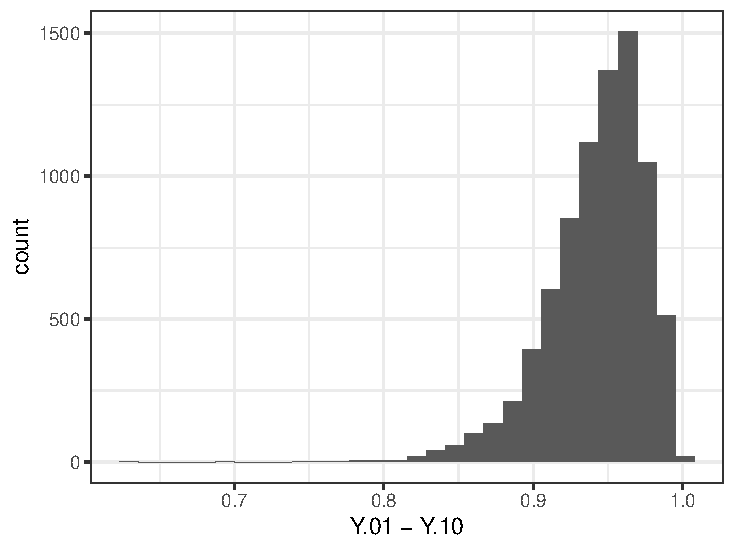
\includegraphics[width=0.6\textwidth,height=\textheight]{paper_files/figure-pdf/fig-posterior-dist-1.pdf}

}

\caption{\label{fig-posterior-dist}Posterior on 'Probability \(Y\) is
increasing in \(X\)'}

\end{figure}

\FloatBarrier

\hypertarget{query-distribution}{%
\subsection{Query distribution}\label{query-distribution}}

\texttt{query\_distribution} works similarly except that distributions
over queries are returned:

\begin{verbatim}
R> make_model("X -> Y") |> 
+  query_distribution(
+    query = list(increasing = "(Y[X=1] > Y[X=0])"), 
+    using = "priors") |>
+  ggplot(aes(increasing)) + geom_histogram() + theme_bw()
\end{verbatim}

\begin{figure}[t]

{\centering \includegraphics[width=0.6\textwidth,height=\textheight]{paper_files/figure-pdf/fig-query-dist-1.pdf}

}

\caption{\label{fig-query-dist}Prior on 'Probability \(Y\) is increasing
in \(X\)'}

\end{figure}

\hypertarget{case-level-queries}{%
\subsection{Case level queries}\label{case-level-queries}}

Sometimes one is interested in assessing the value of a query for a
\emph{particular case}. In a sense this is equivalent to posing a
conditional query, querying conditional on values in a case. For
instance we might consult our posterior lipds model and ask about the
effect of \(X\) on \(Y\) for a case in which \(Z=1, X=1\) and \(Y=1\).

\begin{verbatim}
R> lipids_model |>
+    query_model(query = "Y[X=1] - Y[X=0]",
+              given = c("X==1 & Y==1 & Z==1"),
+              using = "posteriors")
\end{verbatim}

\hypertarget{tbl-case-level-query}{}
\begin{table}[!h]
\caption{\label{tbl-case-level-query}Case Level Quiry Example. }\tabularnewline

\centering
\resizebox{\linewidth}{!}{
\begin{tabular}{cccccc}
\toprule
query & given & mean & sd & cred.low & cred.high\\
\midrule
Y[X=1] - Y[X=0] & X==1 \& Y==1 \& Z==1 & 0.95 & 0.04 & 0.87 & 1\\
\bottomrule
\end{tabular}}
\end{table}

The answer we get in Table~\ref{tbl-case-level-query} is what we now
believe for all cases in which \(Z=1, X=1\) and \(Y=1\). It is in fact
the expected average effect among cases with this data type and so this
expectation has an uncertainty attached to it.

Subtly though this is, in principle, different to what we would infer
for a ``new case'' that we wonder about. When inquirying about a new
case, the case level query \emph{updates} on the given information
observed in the new case. The resulting inference is different to the
inference that would be made from the posterior \emph{given} the
features of the case.

To illustrate, consider a model for which we are quite sure that \(X\)
causes \(Y\) but we do not know whether it works through two positive
effects or two negative effects.

Thus we do not know if M=0 would suggest an effect or no effect. If
asked what we would infer for a case that had \(M=0\) we would not know
whether \(M=0\) information is consistent with a positive effect or not.
However if provided with a randomly case and learn that it has \(M=0\),
then we update about the causal model and infer that there is an effect
in this case (but that there wouldn't be were \(M=1\)).

\begin{verbatim}
R> # DO ALL THIS IN ONE TABLE
R> 
R> set.seed(1)
R>  model <-
+   make_model("X -> M -> Y") |>
+   update_model(data.frame(X = rep(0:1, 8), Y = rep(0:1, 8)), iter = 10000)
R> 
R>  Q <- "Y[X=1] > Y[X=0]"
R>  G <- "X==1 & Y==1 & M==1"
R>  QG <- "(Y[X=1] > Y[X=0]) & (X==1 & Y==1 & M==1)"
R> 
R>  # In this case these are very different:
R>  query_distribution(model, Q, given = G, using = "posteriors")[[1]] |> mean()
R>  query_distribution(model, Q, given = G, using = "posteriors",
+   case_level = TRUE)
R> 
R>  # These are equivalent:
R>  # 1. Case level query via function
R>  query_distribution(model, Q, given = G,
+    using = "posteriors", case_level = TRUE)
R> 
R>  # 2. Case level query by hand using Bayes
R>  distribution <- query_distribution(
+    model, list(QG = QG, G = G), using = "posteriors")
R> 
R>  mean(distribution$QG)/mean(distribution$G)
\end{verbatim}

\hypertarget{batch-queries}{%
\subsection{Batch queries}\label{batch-queries}}

The \texttt{query\_model()} function takes causal queries and conditions
(\texttt{given}) and specifies the parameters to be used. The result is
a data frame which can be displayed as a table.

\begin{verbatim}
R> models <- list(
+ `1` = make_model("X -> Y"),
+ `2` = make_model("X -> Y") |> set_restrictions("Y[X=1] < Y[X=0]")
+ )
R> 
R> query_model(
+  models,
+  query = list(ATE = "Y[X=1] - Y[X=0]", 
+               POS = "Y[X=1] > Y[X=0]"),
+  given = c(TRUE,  "Y==1 & X==1"),
+  case_level = c(FALSE, TRUE),
+  using = c("parameters", "priors"),
+  expand_grid = TRUE)
\end{verbatim}

\hypertarget{tbl-batch-query}{}
\begin{longtable}{ccccccc}
\caption{\label{tbl-batch-query}Results for Two Queries on Two Models. }\tabularnewline

\toprule
model & query & given & using & case\_level & mean & sd\\
\midrule
1 & ATE & - & parameters & FALSE & 0.00 & NA\\
2 & ATE & - & parameters & FALSE & 0.33 & NA\\
1 & ATE & - & priors & FALSE & 0.00 & 0.32\\
2 & ATE & - & priors & FALSE & 0.33 & 0.23\\
1 & ATE & Y==1 \& X==1 & parameters & FALSE & 0.50 & NA\\
2 & ATE & Y==1 \& X==1 & parameters & FALSE & 0.50 & NA\\
1 & ATE & Y==1 \& X==1 & priors & FALSE & 0.50 & 0.29\\
2 & ATE & Y==1 \& X==1 & priors & FALSE & 0.49 & 0.29\\
1 & POS & - & parameters & FALSE & 0.25 & NA\\
2 & POS & - & parameters & FALSE & 0.33 & NA\\
1 & POS & - & priors & FALSE & 0.25 & 0.20\\
2 & POS & - & priors & FALSE & 0.33 & 0.23\\
1 & POS & Y==1 \& X==1 & parameters & FALSE & 0.50 & NA\\
2 & POS & Y==1 \& X==1 & parameters & FALSE & 0.50 & NA\\
1 & POS & Y==1 \& X==1 & priors & FALSE & 0.50 & 0.29\\
2 & POS & Y==1 \& X==1 & priors & FALSE & 0.49 & 0.29\\
1 & ATE & - & parameters & TRUE & 0.00 & NA\\
2 & ATE & - & parameters & TRUE & 0.33 & NA\\
1 & ATE & - & priors & TRUE & 0.00 & NA\\
2 & ATE & - & priors & TRUE & 0.33 & NA\\
1 & ATE & Y==1 \& X==1 & parameters & TRUE & 0.50 & NA\\
2 & ATE & Y==1 \& X==1 & parameters & TRUE & 0.50 & NA\\
1 & ATE & Y==1 \& X==1 & priors & TRUE & 0.50 & NA\\
2 & ATE & Y==1 \& X==1 & priors & TRUE & 0.49 & NA\\
1 & POS & - & parameters & TRUE & 0.25 & NA\\
2 & POS & - & parameters & TRUE & 0.33 & NA\\
1 & POS & - & priors & TRUE & 0.25 & NA\\
2 & POS & - & priors & TRUE & 0.33 & NA\\
1 & POS & Y==1 \& X==1 & parameters & TRUE & 0.50 & NA\\
2 & POS & Y==1 \& X==1 & parameters & TRUE & 0.50 & NA\\
1 & POS & Y==1 \& X==1 & priors & TRUE & 0.50 & NA\\
2 & POS & Y==1 \& X==1 & priors & TRUE & 0.49 & NA\\
\bottomrule
\end{longtable}

\FloatBarrier

\hypertarget{computational-details-and-software-requirements}{%
\section*{Computational details and software
requirements}\label{computational-details-and-software-requirements}}
\addcontentsline{toc}{section}{Computational details and software
requirements}

\begin{longtable}[]{@{}
  >{\raggedleft\arraybackslash}p{(\columnwidth - 4\tabcolsep) * \real{0.1800}}
  >{\centering\arraybackslash}p{(\columnwidth - 4\tabcolsep) * \real{0.4100}}
  >{\raggedright\arraybackslash}p{(\columnwidth - 4\tabcolsep) * \real{0.4100}}@{}}
\toprule()
\endhead
Version & \begin{minipage}[t]{\linewidth}\centering
\begin{itemize}
\tightlist
\item
  1.0.1
\end{itemize}
\end{minipage} & \\
Availability & \begin{minipage}[t]{\linewidth}\centering
\begin{itemize}
\tightlist
\item
  Stable Release:
  https://cran.rstudio.com/web/packages/CausalQueries/index.html
\item
  Development: https://github.com/integrated-inferences/CausalQueries
\end{itemize}
\end{minipage} & \\
Issues & \begin{minipage}[t]{\linewidth}\centering
\begin{itemize}
\tightlist
\item
  https://github.com/integrated-inferences/CausalQueries/issues
\end{itemize}
\end{minipage} & \\
Operating Systems & \begin{minipage}[t]{\linewidth}\centering
\begin{itemize}
\tightlist
\item
  Linux
\item
  MacOS
\item
  Windows
\end{itemize}
\end{minipage} & \\
Testing Environments OS & \begin{minipage}[t]{\linewidth}\centering
\begin{itemize}
\tightlist
\item
  Ubuntu 22.04.2
\item
  Debian 12.2
\item
  MacOS
\item
  Windows
\end{itemize}
\end{minipage} & \\
Testing Environments R & \begin{minipage}[t]{\linewidth}\centering
\begin{itemize}
\tightlist
\item
  R 4.3.1
\item
  R 4.3.0
\item
  R 4.2.3
\item
  r-devel
\end{itemize}
\end{minipage} & \\
R Version & \begin{minipage}[t]{\linewidth}\centering
\begin{itemize}
\tightlist
\item
  R(\textgreater= 3.4.0)
\end{itemize}
\end{minipage} & \\
Compiler & \begin{minipage}[t]{\linewidth}\centering
\begin{itemize}
\tightlist
\item
  either of the below or similar:
\item
  g++
\item
  clang++
\end{itemize}
\end{minipage} & \\
Stan requirements & \begin{minipage}[t]{\linewidth}\centering
\begin{itemize}
\tightlist
\item
  inline
\item
  Rcpp (\textgreater= 0.12.0)
\item
  RcppEigen (\textgreater= 0.3.3.3.0)
\item
  RcppArmadillo (\textgreater= 0.12.6.4.0)
\item
  RcppParallel (\textgreater= 5.1.4)
\item
  BH (\textgreater= 1.66.0)
\item
  StanHeaders (\textgreater= 2.26.0)
\item
  rstan (\textgreater= 2.26.0)
\end{itemize}
\end{minipage} & \\
R-Packages Depends & \begin{minipage}[t]{\linewidth}\centering
\begin{itemize}
\tightlist
\item
  dplyr
\item
  methods
\end{itemize}
\end{minipage} & \\
R-Packages Imports & \begin{minipage}[t]{\linewidth}\centering
\begin{itemize}
\tightlist
\item
  dagitty (\textgreater= 0.3-1)
\item
  dirmult (\textgreater= 0.1.3-4)
\item
  stats (\textgreater= 4.1.1)
\item
  rlang (\textgreater= 0.2.0)
\item
  rstan (\textgreater= 2.26.0)
\item
  rstantools (\textgreater= 2.0.0)
\item
  stringr (\textgreater= 1.4.0)
\item
  ggdag (\textgreater= 0.2.4)
\item
  latex2exp (\textgreater= 0.9.4)
\item
  ggplot2 (\textgreater= 3.3.5)
\item
  lifecycle (\textgreater= 1.0.1)
\end{itemize}
\end{minipage} & \\
\bottomrule()
\end{longtable}

The results in this paper were obtained using
\proglang{R}\textasciitilde3.4.1 with the
\pkg{MASS}\textasciitilde7.3.47 package. \proglang{R} itself and all
packages used are available from the Comprehensive \proglang{R} Archive
Network (CRAN) at {[}https://CRAN.R-project.org/{]}.

\hypertarget{acknowledgments}{%
\section*{Acknowledgments}\label{acknowledgments}}
\addcontentsline{toc}{section}{Acknowledgments}

\begin{tcolorbox}[enhanced jigsaw, breakable, colback=white, opacityback=0, leftrule=.75mm, toprule=.15mm, left=2mm, colframe=quarto-callout-color-frame, arc=.35mm, rightrule=.15mm, bottomrule=.15mm]

The approach to generating a generic stan function that can take data
from arbitrary models was developed in key contributions by
\href{http://jasper-cooper.com/}{Jasper Cooper} and
\href{http://gsyunyaev.com/}{Georgiy Syunyaev}.
\href{https://lilymedina.github.io/}{Lily Medina} did magical work
pulling it all together and developing approaches to characterizing
confounding and defining estimands. Clara Bicalho helped figure out the
syntax for causal statements. Julio Solis made many key contributions
figuring out how to simplify the specification of priors. Merlin
Heidemanns figured out the \texttt{rstantools} integration and made
myriad code improvements. Till Tietz revamped the entire package and
improved every part of it.

\end{tcolorbox}

\hypertarget{references}{%
\section*{References}\label{references}}
\addcontentsline{toc}{section}{References}

\hypertarget{refs}{}
\begin{CSLReferences}{0}{0}
\end{CSLReferences}

\newpage{}

\hypertarget{sec-techdetails}{%
\section*{More technical details}\label{sec-techdetails}}
\addcontentsline{toc}{section}{More technical details}

\begin{tcolorbox}[enhanced jigsaw, breakable, colback=white, opacityback=0, leftrule=.75mm, toprule=.15mm, left=2mm, colframe=quarto-callout-color-frame, arc=.35mm, rightrule=.15mm, bottomrule=.15mm]

Appendices can be included after the bibliography (with a page break).
Each section within the appendix should have a proper section title
(rather than just \emph{Appendix}).

For more technical style details, please check out JSS's style FAQ at
{[}https://www.jstatsoft.org/pages/view/style\#frequently-asked-questions{]}
which includes the following topics:

\begin{itemize}
\tightlist
\item
  Title vs.~sentence case.
\item
  Graphics formatting.
\item
  Naming conventions.
\item
  Turning JSS manuscripts into \proglang{R} package vignettes.
\item
  Trouble shooting.
\item
  Many other potentially helpful details\ldots{}
\end{itemize}

\end{tcolorbox}

\hypertarget{sec-bibtex}{%
\section*{Using BibTeX}\label{sec-bibtex}}
\addcontentsline{toc}{section}{Using BibTeX}

\begin{tcolorbox}[enhanced jigsaw, breakable, colback=white, opacityback=0, leftrule=.75mm, toprule=.15mm, left=2mm, colframe=quarto-callout-color-frame, arc=.35mm, rightrule=.15mm, bottomrule=.15mm]

References need to be provided in a \textsc{Bib}{\TeX} file
(\texttt{.bib}). All references should be made with \texttt{@cite}
syntax. This commands yield different formats of author-year citations
and allow to include additional details (e.g.,pages, chapters, \dots) in
brackets. In case you are not familiar with these commands see the JSS
style FAQ for details.

Cleaning up \textsc{Bib}{\TeX} files is a somewhat tedious task --
especially when acquiring the entries automatically from mixed online
sources. However, it is important that informations are complete and
presented in a consistent style to avoid confusions. JSS requires the
following format.

\begin{itemize}
\tightlist
\item
  item JSS-specific markup (\texttt{\textbackslash{}proglang},
  \texttt{\textbackslash{}pkg}, \texttt{\textbackslash{}code}) should be
  used in the references.
\item
  item Titles should be in title case.
\item
  item Journal titles should not be abbreviated and in title case.
\item
  item DOIs should be included where available.
\item
  item Software should be properly cited as well. For \proglang{R}
  packages \texttt{citation("pkgname")} typically provides a good
  starting point.
\end{itemize}

\end{tcolorbox}

\hypertarget{appendix-stan-code}{%
\section{Appendix: stan code}\label{appendix-stan-code}}

\texttt{prep\_stan\_data} then returns a list of objects that
\texttt{stan} expects to receive. These include indicators to figure out
where a parameter set starts (\texttt{l\_starts}, \texttt{l\_ends}) and
ends and where a data strategy starts and ends
(\texttt{strategy\_starts}, \texttt{strategy\_ends}), as well as the
matrices described above.

MOVE TO APPENDIX? ADD DISCUSSION OF PARMAP

Below we show the \texttt{stan} code. This starts off with a block
saying what input data is to be expected. Then there is a
characterization of parameters and the transformed parameters. Then the
likelihoods and priors are provided. \texttt{stan} takes it from there
and generates a posterior distribution.

\begin{verbatim}
#> functions{
#>   row_vector col_sums(matrix X) {
#>     row_vector[cols(X)] s ;
#>     s = rep_row_vector(1, rows(X)) * X ;
#>     return s ;
#>   }
#> }
#> data {
#> int<lower=1> n_params;
#> int<lower=1> n_paths;
#> int<lower=1> n_types;
#> int<lower=1> n_param_sets;
#> int<lower=1> n_nodes;
#> array[n_param_sets] int<lower=1> n_param_each;
#> int<lower=1> n_data;
#> int<lower=1> n_events;
#> int<lower=1> n_strategies;
#> int<lower=0, upper=1> keep_transformed;
#> vector<lower=0>[n_params] lambdas_prior;
#> array[n_param_sets] int<lower=1> l_starts;
#> array[n_param_sets] int<lower=1> l_ends;
#> array[n_nodes] int<lower=1> node_starts;
#> array[n_nodes] int<lower=1> node_ends;
#> array[n_strategies] int<lower=1> strategy_starts;
#> array[n_strategies] int<lower=1> strategy_ends;
#> matrix[n_params, n_types] P;
#> matrix[n_params, n_paths] parmap;
#> matrix[n_paths, n_data] map;
#> matrix<lower=0,upper=1>[n_events,n_data] E;
#> array[n_events] int<lower=0> Y;
#> }
#> parameters {
#> vector<lower=0>[n_params - n_param_sets] gamma;
#> }
#> transformed parameters {
#> vector<lower=0, upper=1>[n_params] lambdas;
#> vector<lower=1>[n_param_sets] sum_gammas;
#> matrix[n_params, n_paths] parlam;
#> matrix[n_nodes, n_paths] parlam2;
#> vector<lower=0, upper=1>[n_paths] w_0;
#> vector<lower=0, upper=1>[n_data] w;
#> vector<lower=0, upper=1>[n_events] w_full;
#> // Cases in which a parameter set has only one value need special handling
#> // they have no gamma components and sum_gamma needs to be made manually
#> for (i in 1:n_param_sets) {
#>   if (l_starts[i] >= l_ends[i]) {
#>     sum_gammas[i] = 1;
#>     // syntax here to return unity as a vector
#>     lambdas[l_starts[i]] = lambdas_prior[1]/lambdas_prior[1];
#>     }
#>   else if (l_starts[i] < l_ends[i]) {
#>     sum_gammas[i] =
#>     1 + sum(gamma[(l_starts[i] - (i-1)):(l_ends[i] - i)]);
#>     lambdas[l_starts[i]:l_ends[i]] =
#>     append_row(1, gamma[(l_starts[i] - (i-1)):(l_ends[i] - i)]) /
#>       sum_gammas[i];
#>     }
#>   }
#> // Mapping from parameters to data types
#> // (usual case): [n_par * n_data] * [n_par * n_data]
#> parlam  = rep_matrix(lambdas, n_paths) .* parmap;
#> // Sum probability over nodes on each path
#> for (i in 1:n_nodes) {
#>  parlam2[i,] = col_sums(parlam[(node_starts[i]):(node_ends[i]),]);
#>  }
#> // then take product  to get probability of data type on path
#> for (i in 1:n_paths) {
#>   w_0[i] = prod(parlam2[,i]);
#>  }
#>  // last (if confounding): map to n_data columns instead of n_paths
#>  w = map'*w_0;
#>   // Extend/reduce to cover all observed data types
#>  w_full = E * w;
#> }
#> model {
#> // Dirichlet distributions (earlier versions used gamma)
#> for (i in 1:n_param_sets) {
#>   target += dirichlet_lpdf(lambdas[l_starts[i]:l_ends[i]]  |
#>     lambdas_prior[l_starts[i] :l_ends[i]]);
#>   target += -n_param_each[i] * log(sum_gammas[i]);
#>  }
#> // Multinomials
#> // Note with censoring event_probabilities might not sum to 1
#> for (i in 1:n_strategies) {
#>   target += multinomial_lpmf(
#>   Y[strategy_starts[i]:strategy_ends[i]] |
#>     w_full[strategy_starts[i]:strategy_ends[i]]/
#>      sum(w_full[strategy_starts[i]:strategy_ends[i]]));
#>  }
#> }
#> // Option to export distribution of causal types
#> generated quantities{
#> vector[n_types] prob_of_types;
#> if (keep_transformed == 1){
#> for (i in 1:n_types) {
#>    prob_of_types[i] = prod(P[, i].*lambdas + 1 - P[,i]);
#> }}
#>  if (keep_transformed == 0){
#>     prob_of_types = rep_vector(1, n_types);
#>  }
#> }
\end{verbatim}


  \bibliography{supp/bib.bib}


\end{document}
